\chapter{Architectural Design}

\section{Overview}

The S\&C platform employs a three-tier architecture, a widely adopted design pattern in software development that separates applications into three distinct layers: the presentation layer, the application layer, and the data layer. Each of these layers serves a specific function, contributing to the system’s scalability, maintainability, and flexibility. Below are the details of each layer:

\begin{itemize}
    \item \textbf{Presentation Layer:}  
    This is the user interface (UI) of the application, responsible for how the system is presented to the end-user. It interacts directly with the user, capturing inputs and displaying results. The presentation layer ensures that users can easily access and interact with the system’s functionalities, typically through web browsers, mobile apps, or desktop applications.

    \item \textbf{Application Layer:}  
    Often referred to as the business logic layer, this is where all the processing of data and execution of business rules occurs. It receives requests from the presentation layer, processes the logic, and sends responses back. The application layer is responsible for handling complex operations such as data validation, computations, decision-making processes, and ensuring that data flows smoothly between the user interface and the database.

    \item \textbf{Data Layer:}  
    This layer is responsible for storing, managing, and retrieving data. It typically includes databases, file systems, or other data storage solutions that support the application’s needs. The data layer ensures that all data related to the application—such as user information, transactional records, or application settings—is organized, secured, and accessible when needed. The application layer communicates with this layer to retrieve and update information as required.
\end{itemize}

The primary benefit of this three-tier architecture is that each layer can be developed, maintained, and scaled independently by different development teams. This modular approach allows for better resource management and reduces the complexity of managing the system as a whole. Changes made to one layer, such as updates to the presentation or application logic, can be implemented without affecting the other layers. Additionally, scalability is a significant advantage, as each tier can be scaled up or down independently depending on demand, ensuring optimal performance and resource utilization without impacting the entire system. This separation of concerns also improves maintainability, as each layer can be updated or replaced with minimal disruption to the others.

\section{Component View}

\begin{figure}[H]
    \centering
    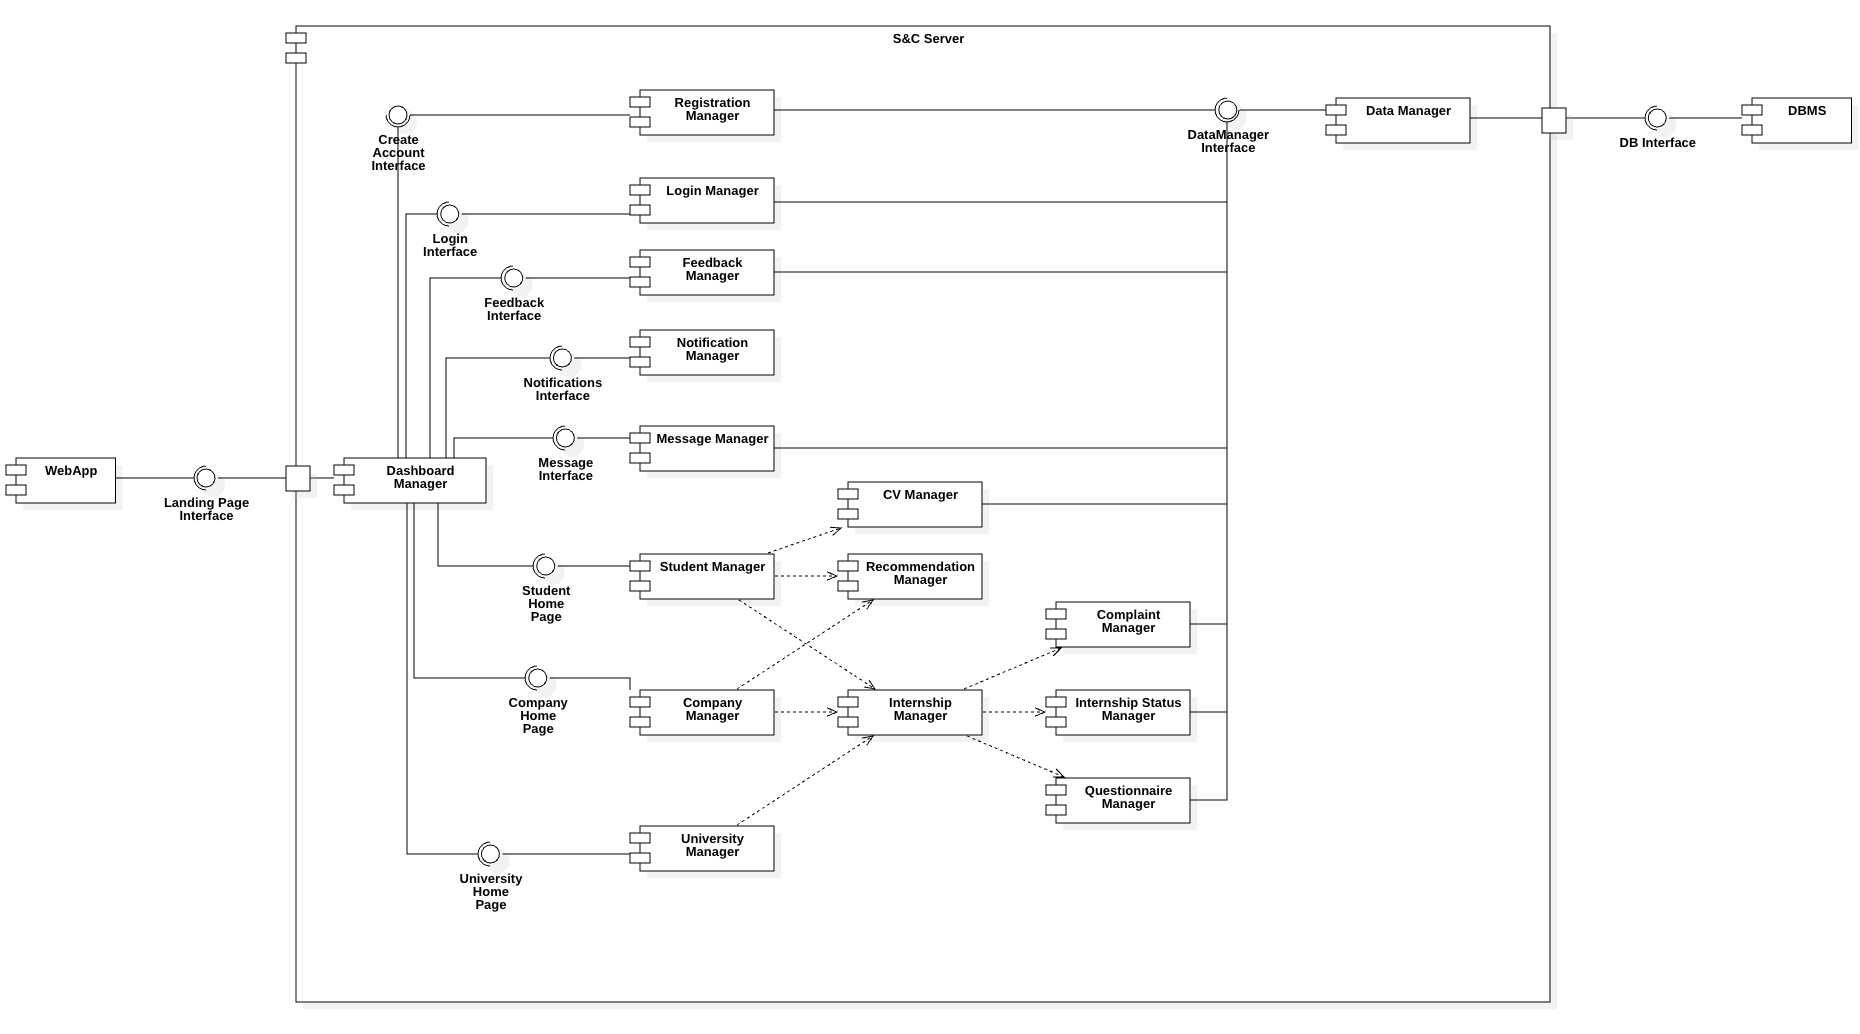
\includegraphics[width=1\linewidth]{DD/Images/component_diagram.png}
    \caption{Component Diagram}
    \label{fig:enter-label}
\end{figure}

\begin{itemize}
    \item \textbf{Dashboard Manager}: It is the pivotal component that orchestrates all communication between users and the S\&C platform. Acting as the central hub for user interactions, it manages all requests routed through the Dashboard Interface. Whether users are registering, applying for internships, or managing their profiles, the Dashboard Manager directs their requests to the appropriate system components. By integrating with other modules, it provides an easy user experience while ensuring efficient communication across the platform.
    \item \textbf{Registration Manager}: it is responsible for handling the registration process for all users on the platform, including students, companies, and universities. It ensures that user data is properly validated and securely stored. The manager also oversees the verification process for universities, ensuring that institutions are properly accredited. Additionally, it manages account recovery workflows and ensures that users activate their accounts correctly.
    \item \textbf{Login Manager}: it handles the login process for registered users. It is responsible for managing user authentication, session management, and ensuring that secure login mechanisms, such as two-factor authentication and CAPTCHA, are implemented. The Login Manager also manages account lockouts, password resets, and controls user access levels to maintain the system's security.
    \item \textbf{Student Manager}: it oversees all functionalities related to students on the platform. This component allows students to update their personal details and manage their profiles. It serves as a point of interaction between students and other modules, such as internships and recommendations. 
    \item \textbf{Company Manager}: it is responsible for managing all company-related functionalities on the platform. It ensures that companies provide complete and accurate details on their profiles and that internship postings are up to date. The Company Manager also assists companies in improving the quality of their internship postings, ensuring they meet the platform's standards and attract the best candidates.
    \item \textbf{University Manager}: it manages the registration and verification of universities on the platform. It provides universities with tools to monitor and track the internships of their affiliated students. The University Manager also facilitates the resolution of complaints, ensuring that internships comply with academic standards and regulations.
     \item \textbf{CV Manager}: it allows students to upload, edit, and enhance their CVs. This module provides suggestions and best practices to help students create impactful CVs and integrates with the Recommendation Manager to improve the content of students' CVs based on feedback received.
    \item \textbf{Internship Manager}: it handles the entire lifecycle of internships, from posting opportunities to completion. It allows companies to post, update, and manage internships and enables students to apply and track their internship status.
    \item \textbf{Internship Status Manager}: it provides comprehensive tracking and management of internship statuses. Beyond simply updating statuses such as "pending," "active," or "completed," it facilitates deeper insights by generating progress reports for universities and companies. It allows stakeholders to review milestones, address any delays, and ensure that internships adhere to expected timelines.
    \item \textbf{Questionnaire Manager}: it distributes and manages feedback forms sent to students and companies. It not only collects and analyzes responses to evaluate internship quality but also uses the insights to suggest actionable improvements. The manager ensures all feedback is utilized to enhance the overall internship experience.
    \item \textbf{Message Manager}: it is responsible for facilitating direct communication among users. This module ensures direct messaging between students, companies, and universities. It integrates with the Notification Manager to notify users of unread messages and supports features such as file sharing and automated replies. The Message Manager also archives communications to ensure accountability and provide a reference for future interactions.
    \item \textbf{Complaint Manager}: it is responsible for handling the submission and resolution of complaints from students, companies, and universities. It ensures that all complaints are properly logged, categorized, and processed in an efficient manner. The Complaint Manager works closely with the University Manager to address any academic-related complaints and ensures that all complaints are handled according to platform policies.
    \item \textbf{Recommendation Manager}: it provides personalized internship recommendations for students based on their CVs and preferences. It also suggests potential candidates to companies based on their internship requirements. The Manager uses keyword-based and statistical analysis to improve the accuracy of recommendations, ensuring that students and companies are paired effectively.
    \item \textbf{Feedback Manager}: it collects and analyzes feedback from users about the platform and its features. It generates actionable insights from the feedback to continuously improve the user experience. This component is crucial for refining CV suggestions, internship postings, and recommendations, ensuring the platform evolves based on user input.
    \item \textbf{Notification Manager}: it handles all notifications and alerts sent to users, such as updates on internship statuses, application statuses, and reminders. It ensures that notifications are sent in a timely and relevant manner through email, SMS, or in-app messages. The Notification Manager also manages user preferences, ensuring that notifications are relevant and that users can customize how and when they receive alerts.
    \item \textbf{Data Manager}: it handles all data storage and retrieval operations, interfacing directly with the DBMS through the DB Interface. It provides a centralized access point for components like the Registration and Internship Managers via the DataManager Interface, ensuring secure, consistent, and efficient data management across the system.
    \item \textbf{Email Manager}: it handles all email related operations, primarily focusing on user verification. It sends account activation emails during registration and manages password recovery emails. It ensures secure and reliable communication between the platform and its users.
\end{itemize}

\section{Deployment View}
\begin{figure}[H]
    \centering
    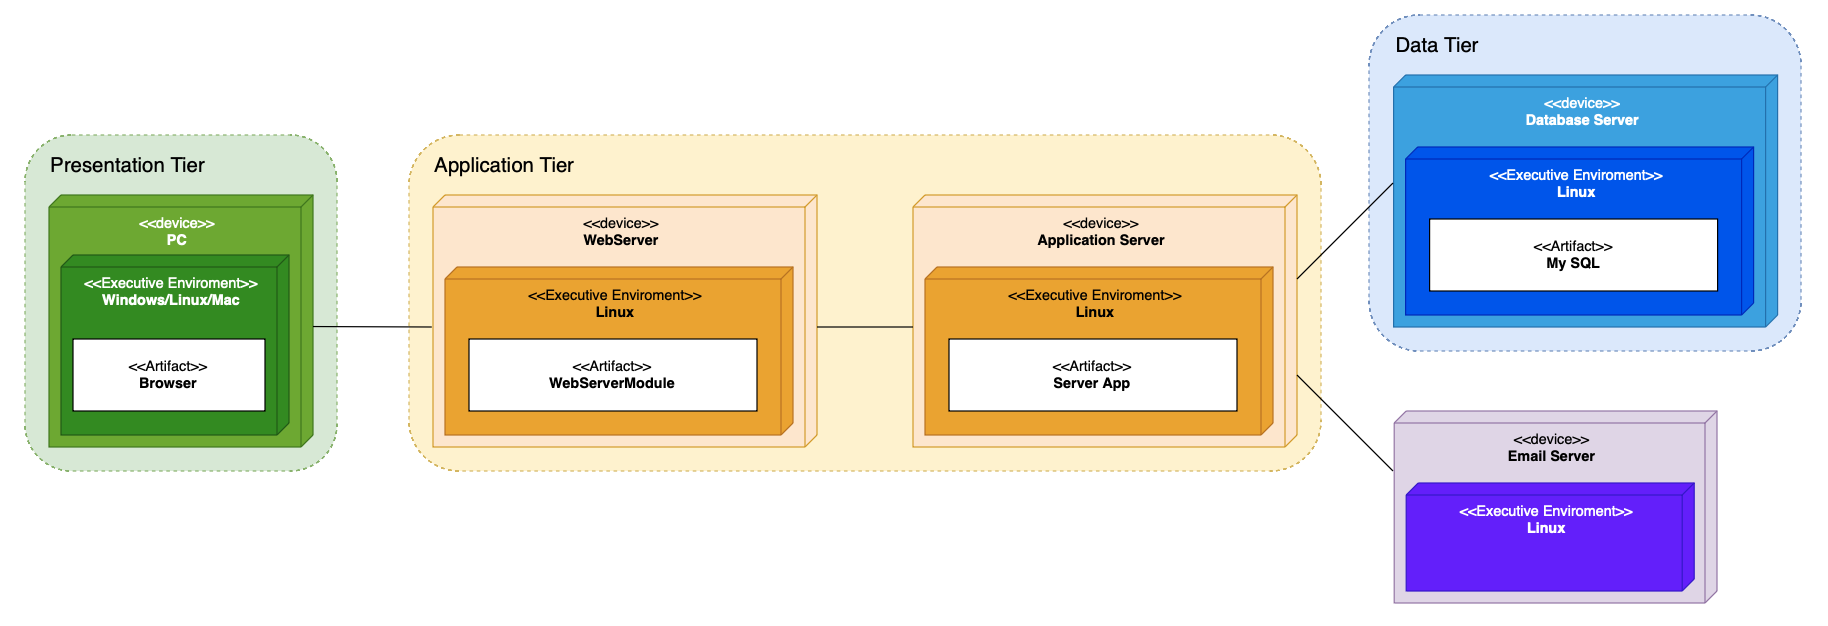
\includegraphics[width=1\linewidth]{DD/Images/deployment_diagram.png}
    \caption{Deployment Diagram}
    \label{fig:enter-label}
\end{figure}
The deployment view presented here is important as it describes the system's execution environment while also illustrating the topological distribution of the application.

The system's deployment architecture ensures efficient operation, scalability, and security across its components. Users can access the system using any personal computer or device with a web browser, such as mobile phones, tablets, or desktops. The browser communicates with the Web Server to send and receive requests.

The Web Server acts as a gateway, handling incoming client requests and performing load balancing to distribute them across multiple Application Servers. It does not execute business logic but instead ensures that traffic is managed efficiently, preventing server overload. The Web Server also provides the necessary HTML, JSON, JavaScript, and CSS files to clients.

A firewall sits between clients and the system to ensure security. It limits access by applying strict rules, protecting the system from potential malicious intrusions and attacks. It also checks for any suspicious requests before they reach the server.

The Application Server is the heart of the system's business logic. It manages requests from the Web Server, routing them to the appropriate module through the Dashboard Manager. The Application Server communicates with the Database Server via a model gateway, ensuring that any changes to the database are processed and updated via TCP/IP. It is replicated to handle large user traffic and ensure system scalability.

The Database Server stores and manages critical system data using MySQL. The Application Server retrieves and updates this data through the model module and database driver to maintain data consistency.

After registration, users must confirm their accounts by clicking a verification link sent via email. The Application Server contacts the Email Server using the SMTP protocol to send the confirmation email immediately after the registration process, ensuring secure user verification.


\newpage
\section{Runtime View}

\subsection{User Registration}
\begin{figure} [H]
    \centering
    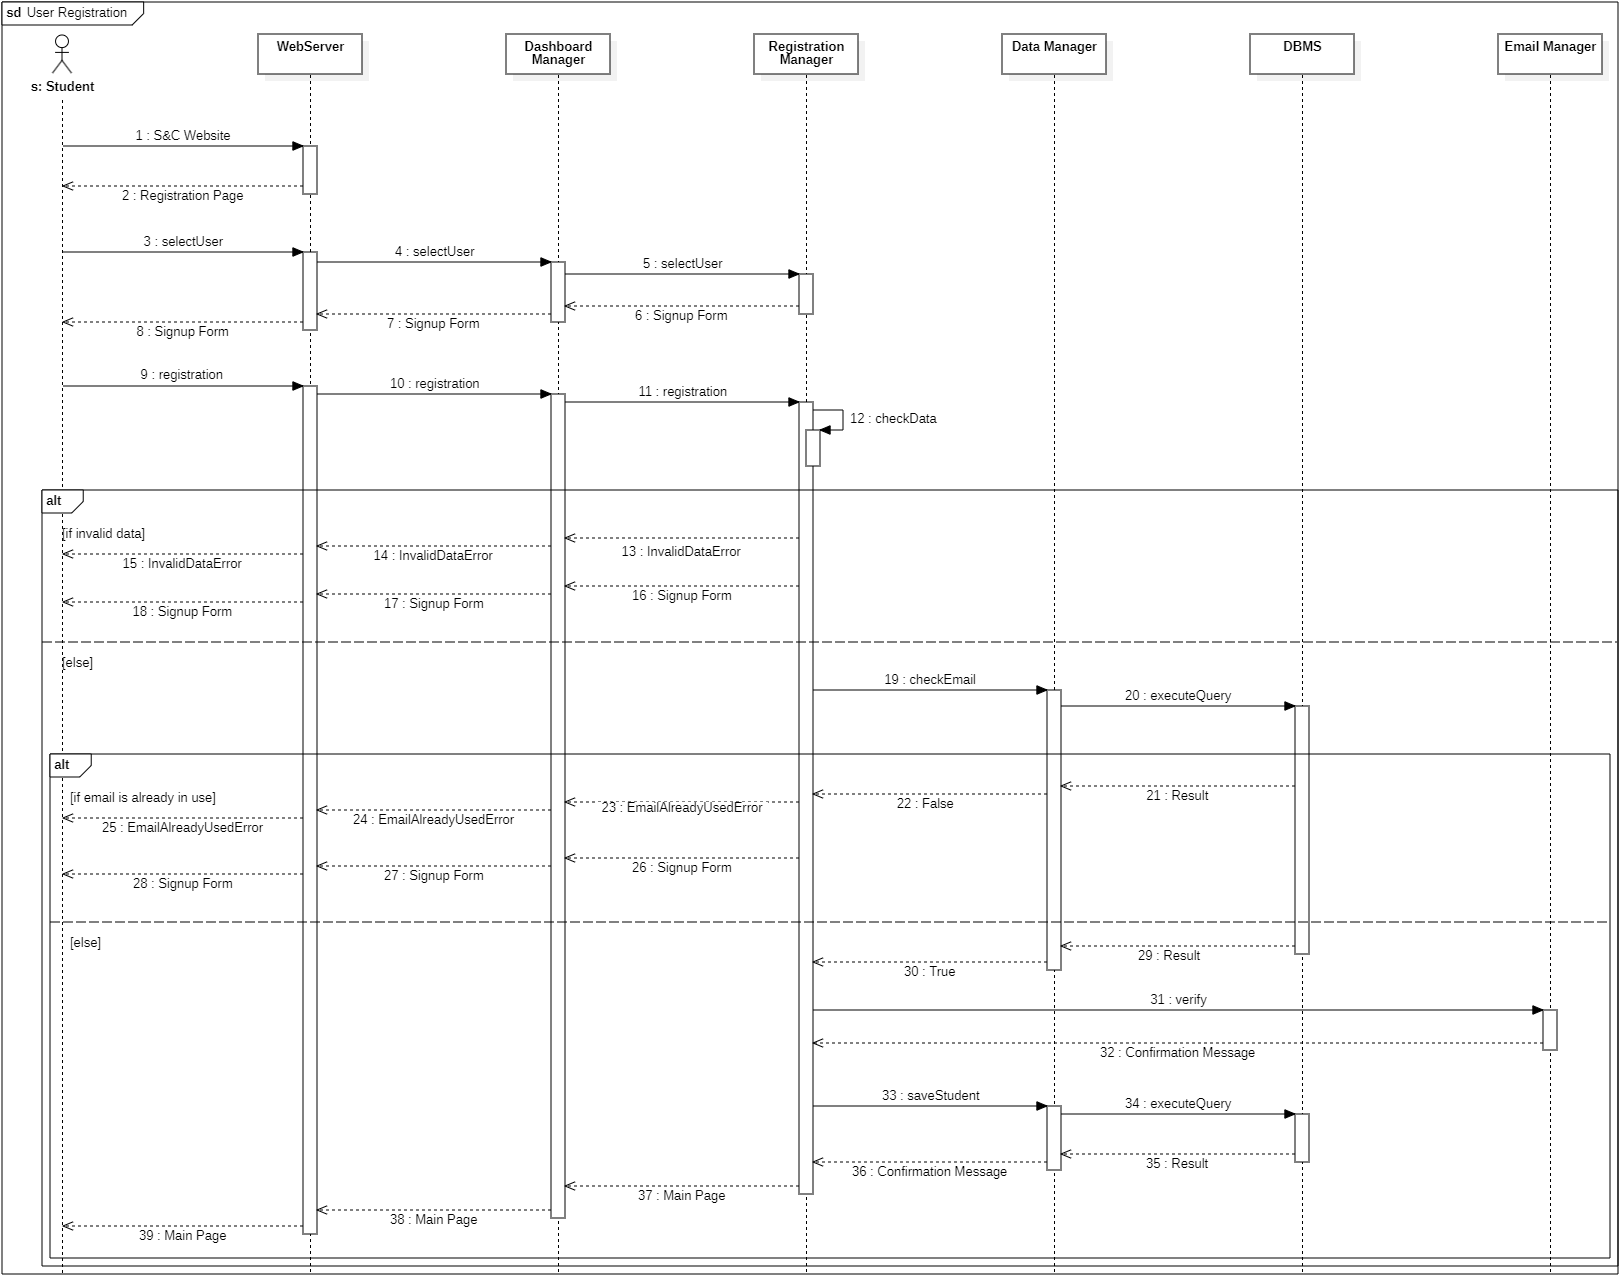
\includegraphics[width=1\linewidth]{DD/Images/Runtime Sequence Diagram Images/user_registration.png}
    \caption{Diagram for [UC1]}
    \label{fig: User Registration Diagram}
\end{figure}
The user registration process begins with the user selecting their role (student, company, or university) and accessing the signup form. The form requires personal details, such as name, email, and password, and additional information based on the role. Once the data is submitted, the system validates its completeness and verifies whether the email is already in use. Errors prompt the user to revise their input. If the data passes validation, the system saves the information, sends a verification email, and redirects the user to the main page. This process ensures secure and role-specific onboarding for all types of users.

\subsection{User Login}
\begin{figure} [H]
    \centering
    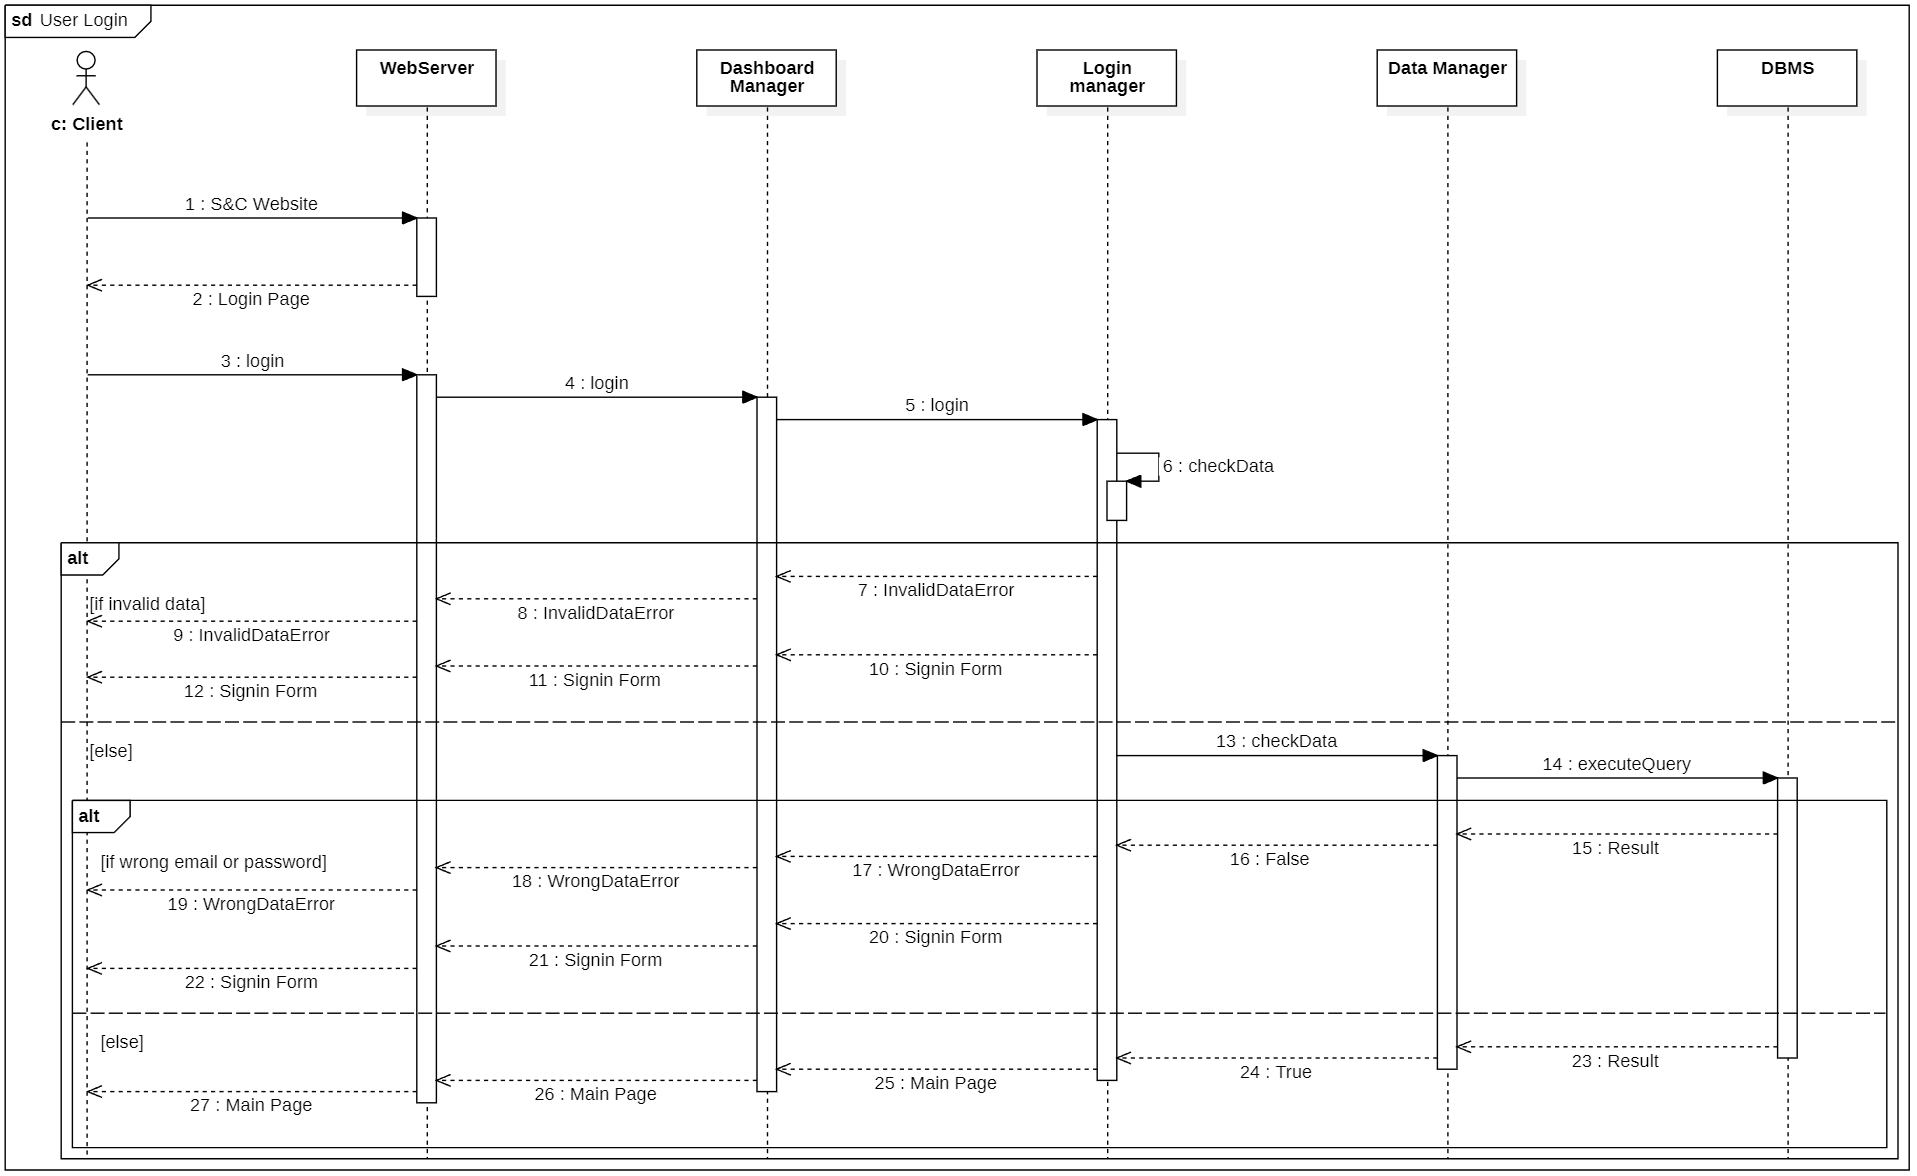
\includegraphics[width=1\linewidth]{DD/Images/Runtime Sequence Diagram Images/user_login.png}
    \caption{Diagram for [UC2]}
    \label{fig: User Login Diagram}
\end{figure}
This diagram outlines the user login process on the platform. The user accesses the login page and submits their email and password. The system validates the input, checking for completeness and correctness. If any issues are found, such as missing fields or invalid credentials, an error message is displayed, guiding the user to resolve the problem. If the credentials are valid, the system authenticates the user and grants access to the main dashboard. For invalid email-password combinations, specific error feedback is provided to avoid confusion and streamline the login experience.

\subsection{Insert CV Information}
\begin{figure} [H]
    \centering
    \includegraphics[width=1\linewidth]{DD/Images/Runtime Sequence Diagram Images/insert_cv_information.png}
    \caption{Diagram for [UC3]}
    \label{fig: Insert CV Information Diagram}
\end{figure}
This diagram describes how a student adds their CV information to the platform. The student accesses the CV insertion form, where they input details such as education, skills, and work experience. The system validates the data for completeness and accuracy. If errors are found, an error message prompts corrections. For valid inputs, the system provides improvement suggestions to optimize the CV’s presentation. Once finalized, the CV is saved in the database, and the student receives a confirmation message. This ensures students can maintain professional, high-quality CVs.

\subsection{Update CV Information}
\begin{figure} [H]
    \centering
    \includegraphics[width=1\linewidth]{DD/Images/Runtime Sequence Diagram Images/update_cv_information.png}
    \caption{Diagram for [UC4]}
    \label{fig: Update CV Information Diagram}
\end{figure}
This diagram describes how a student updates their CV on the platform. The student selects their CV, views its current details, and accesses the update form to modify fields like education, skills, or work experience. Once submitted, the system validates the input for completeness and correctness, providing feedback on any errors. If the data is valid, the system may offer suggestions to further improve the CV’s structure or content. After finalization, the updated CV is saved to the database, and a confirmation message is sent to the student. This process ensures students maintain accurate and competitive CVs on the platform.

\subsection{Create Internship}
\begin{figure} [H]
    \centering
    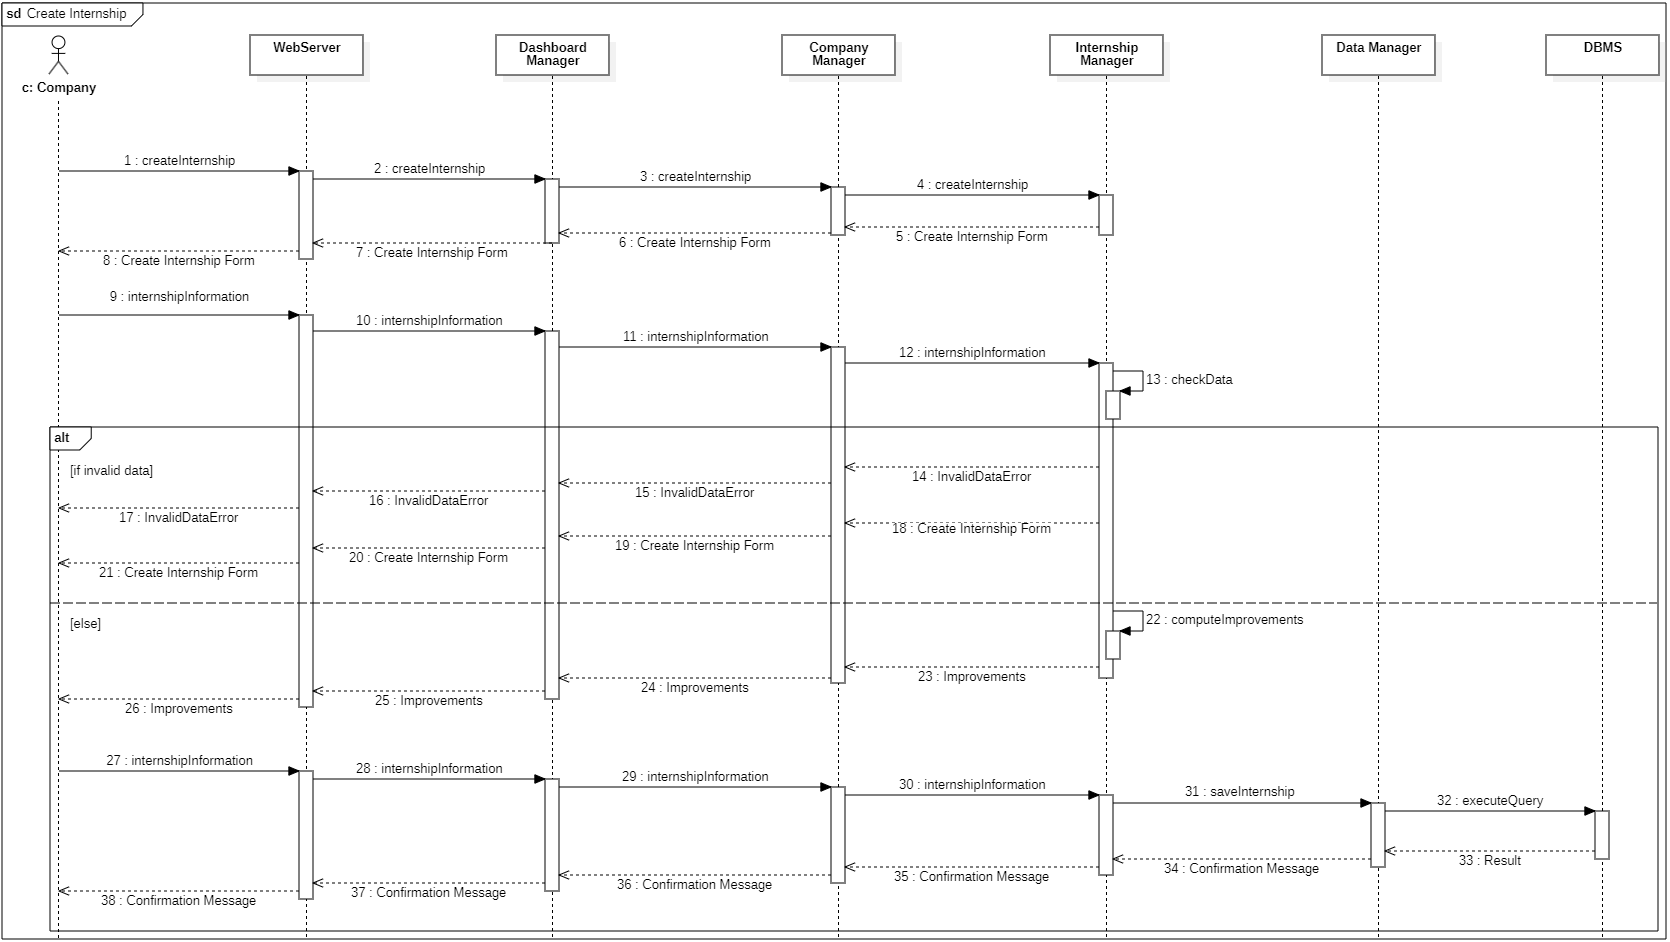
\includegraphics[width=1\linewidth]{DD/Images/Runtime Sequence Diagram Images/create_internship.png}
    \caption{Diagram for [UC5]}
    \label{fig: Create Internship Diagram}
\end{figure}
This diagram explains how a company creates a new internship listing. The company begins by accessing the internship creation form, where they input details like the internship name, description, deadline, and requirements. After submitting the form, the system validates the input. If errors are detected, the system provides feedback for corrections. For valid data, improvement suggestions may be offered to optimize the internship posting. Once finalized, the internship is saved in the database, and a confirmation message is sent to the company. The process ensures that internships are detailed, accurate, and aligned with platform standards.

\subsection{Update Internship}
\begin{figure} [H]
    \centering
    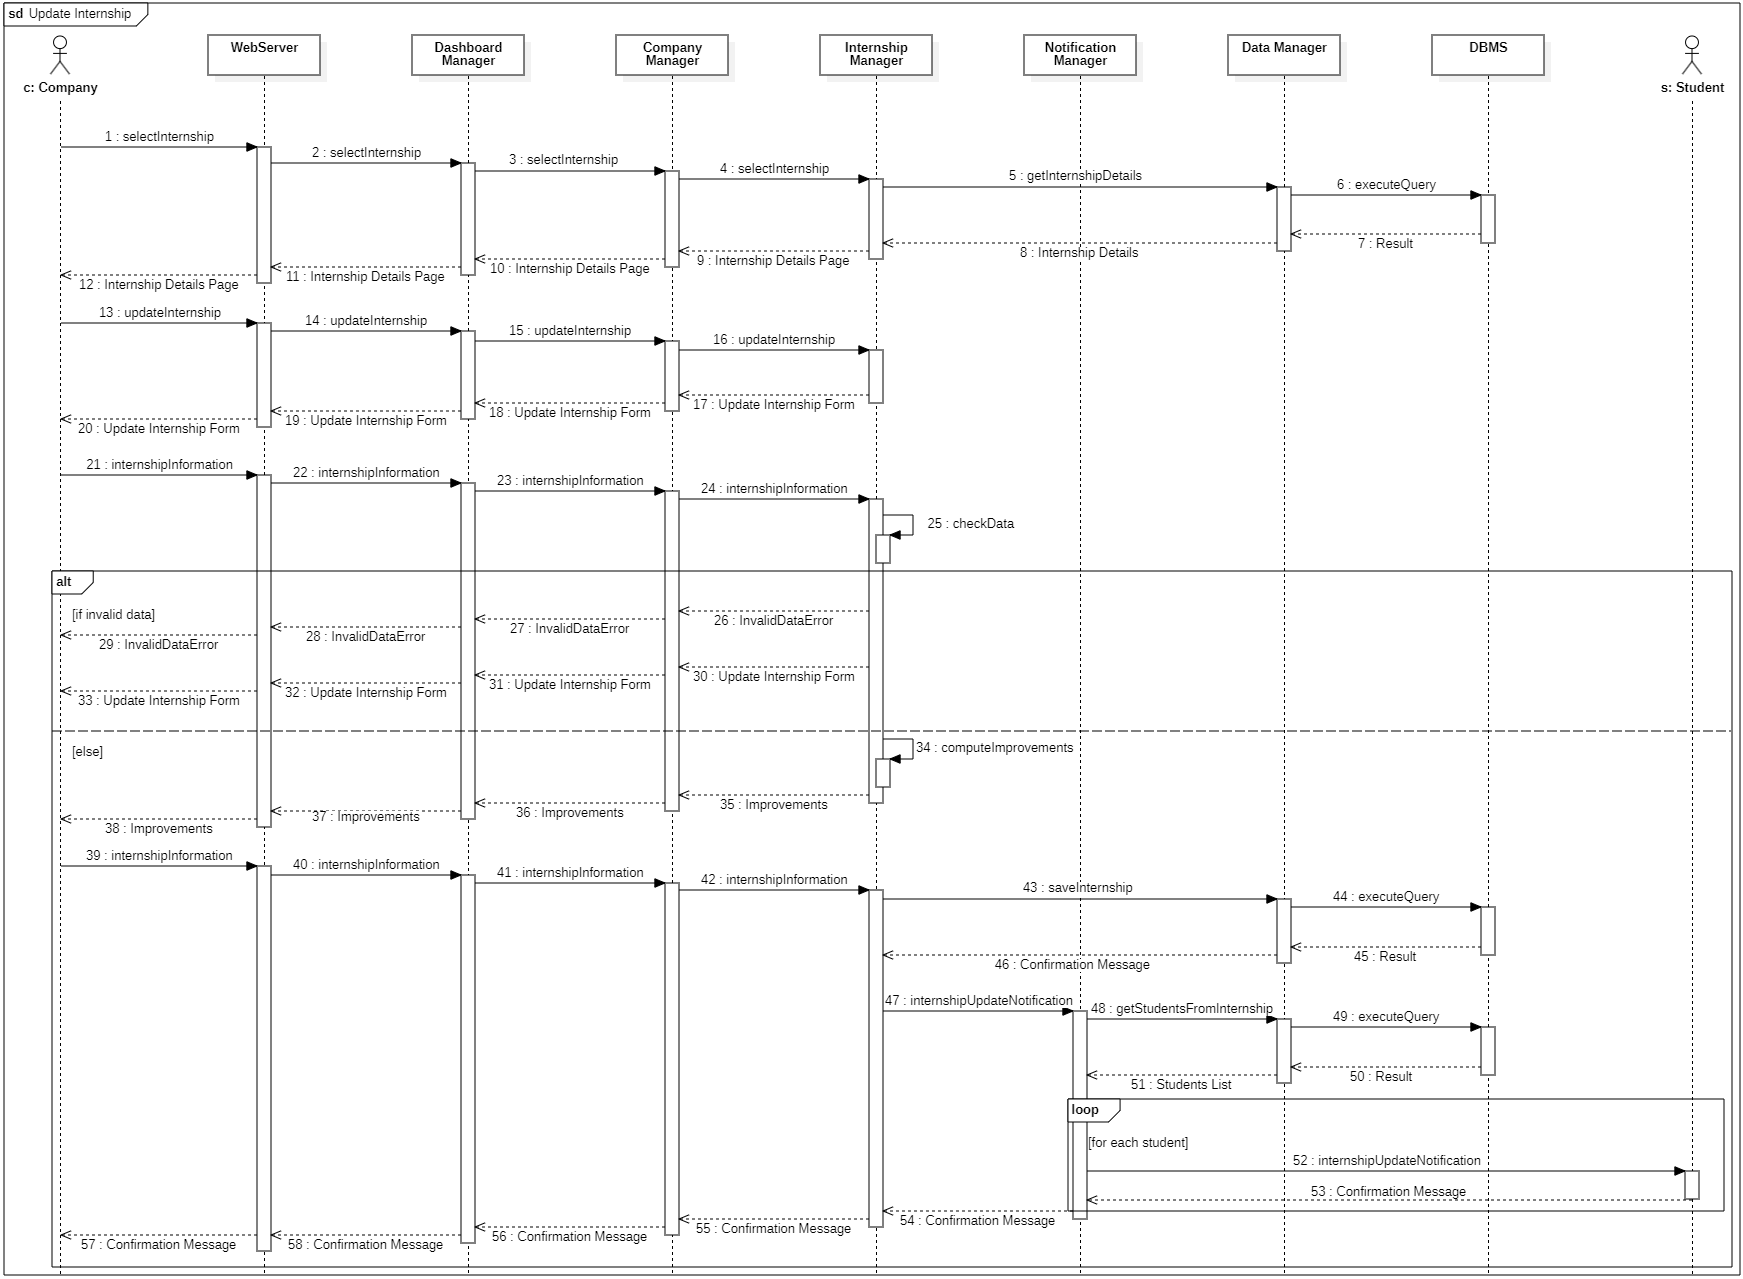
\includegraphics[width=1\linewidth]{DD/Images/Runtime Sequence Diagram Images/update_internship.png}
    \caption{Diagram for [UC6]}
    \label{fig: Update Internship Diagram}
\end{figure}

This diagram illustrates the process for a company to update an internship listing. The company begins by selecting the internship to edit, and the system retrieves its details. After making changes, the company submits the updated information, which the system validates for completeness and accuracy. If errors are detected, the system displays a message prompting corrections. If valid, the system may suggest improvements to refine the listing, such as clarifying descriptions or adjusting deadlines. Once the updates are finalized, the information is saved in the database. Notifications are sent to all students associated with the internship, informing them of the changes and maintaining transparency.

\subsection{Search Internship}
\begin{figure} [H]
    \centering
    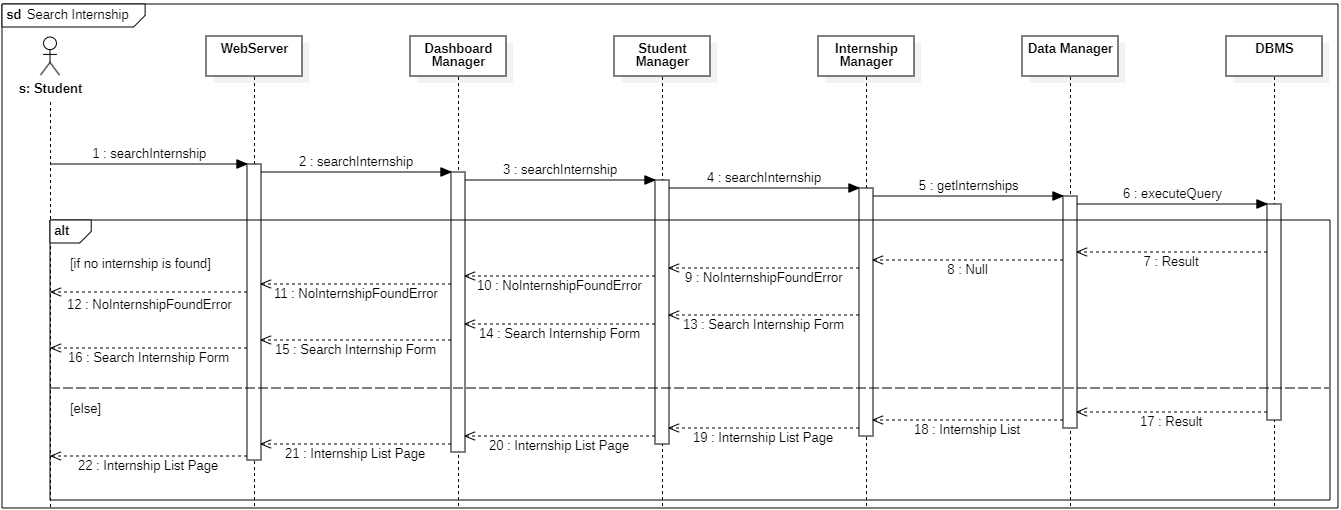
\includegraphics[width=1\linewidth]{DD/Images/Runtime Sequence Diagram Images/search_internship.png}
    \caption{Diagram for [UC7]}
    \label{fig: Search Internship Diagram}
\end{figure}

This sequence diagram depicts how a student searches for internships on the platform. The student provides search criteria, such as keywords, deadlines, or required skills, which the system uses to query the database. If no matches are found, the system displays an error and suggests refining the search. If matches are found, a list of internships is returned, allowing the student to browse through opportunities. This process ensures that students can efficiently find internships that align with their preferences and qualifications, facilitating their journey toward securing practical experience.

\subsection{Submit Application}
\begin{figure} [H]
    \centering
    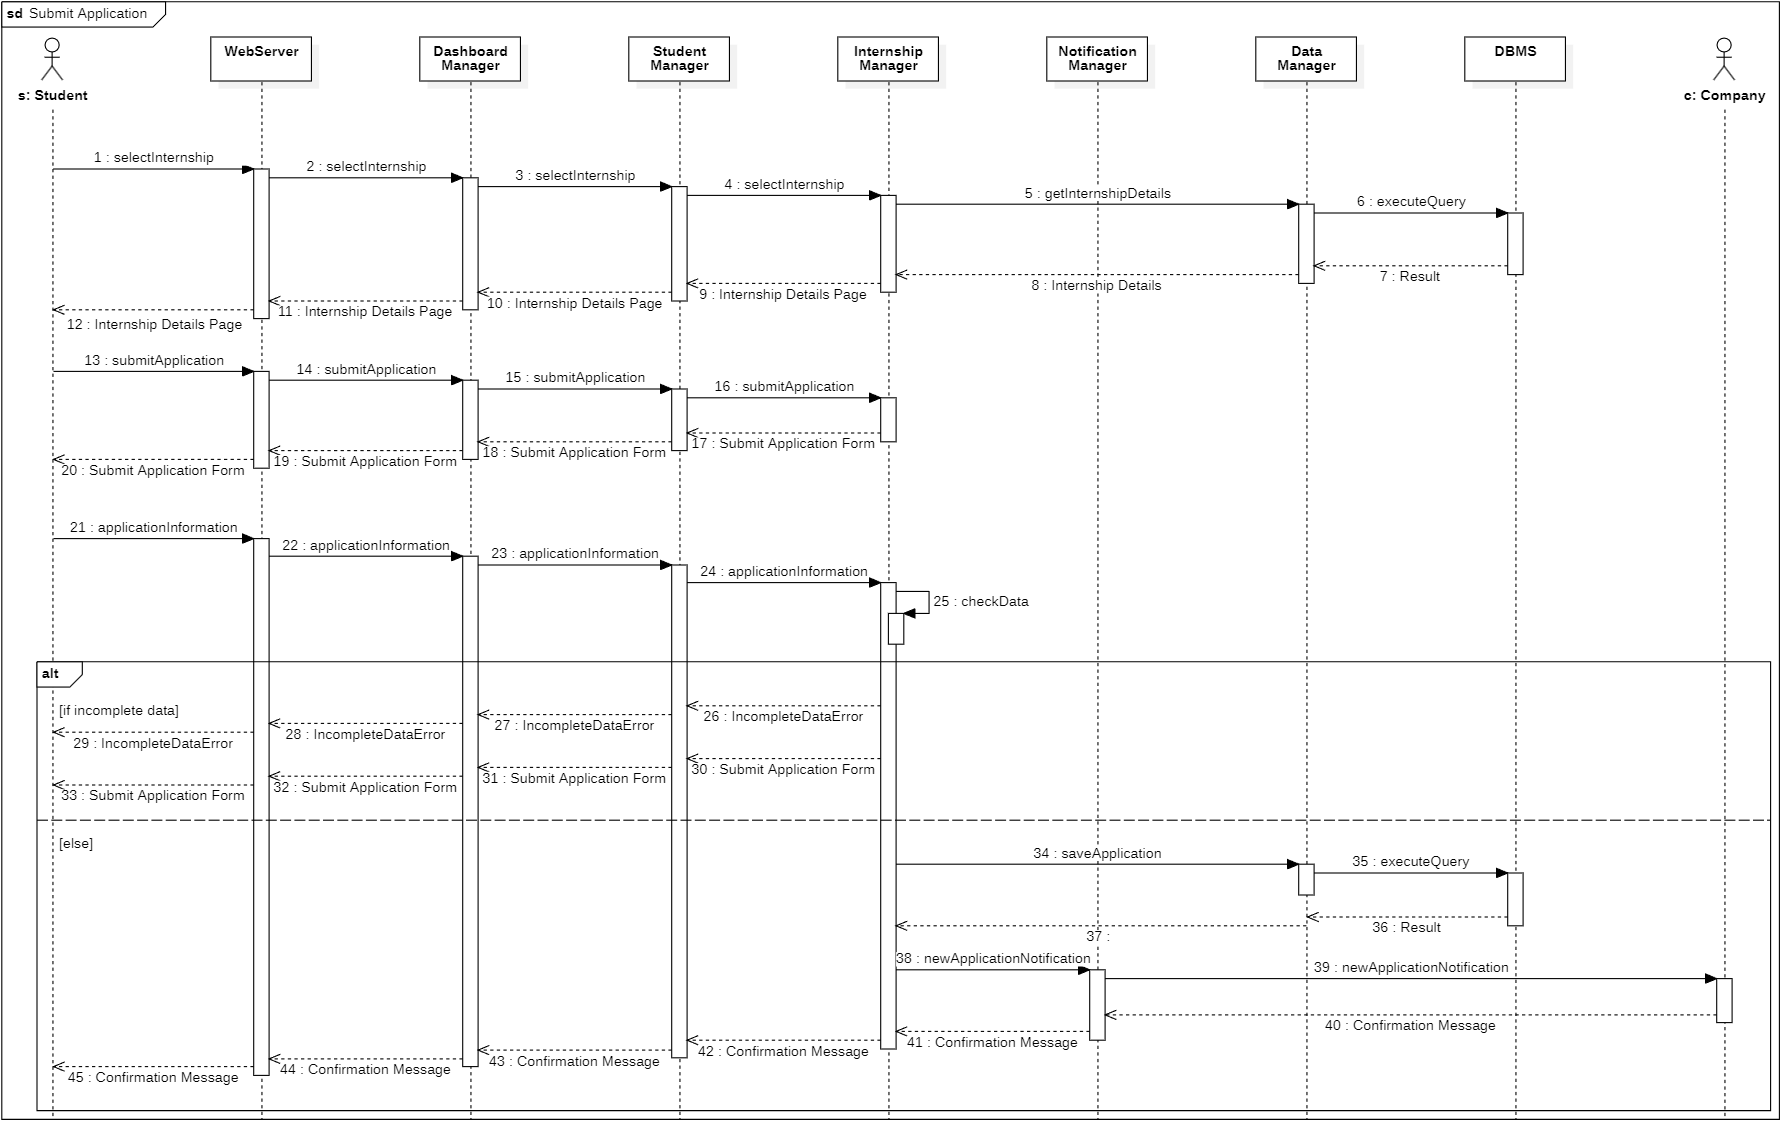
\includegraphics[width=1\linewidth]{DD/Images/Runtime Sequence Diagram Images/submit_application.png}
    \caption{Diagram for [UC8]}
    \label{fig: Submit Application Diagram}
\end{figure}
The diagram explains how a student submits an application for an internship. After selecting an internship, the student views its details and accesses the application form. They fill out the required fields, such as a cover letter or additional details, and submit the form. The system validates the input, ensuring all fields are complete and free of errors. If valid, the application is saved in the database, and the company offering the internship is notified. The student receives a confirmation message, ensuring transparency and completion of the process. This facilitates an easy application experience for both students and companies.

\subsection{Insert Questionnaire}
\begin{figure} [H]
    \centering
    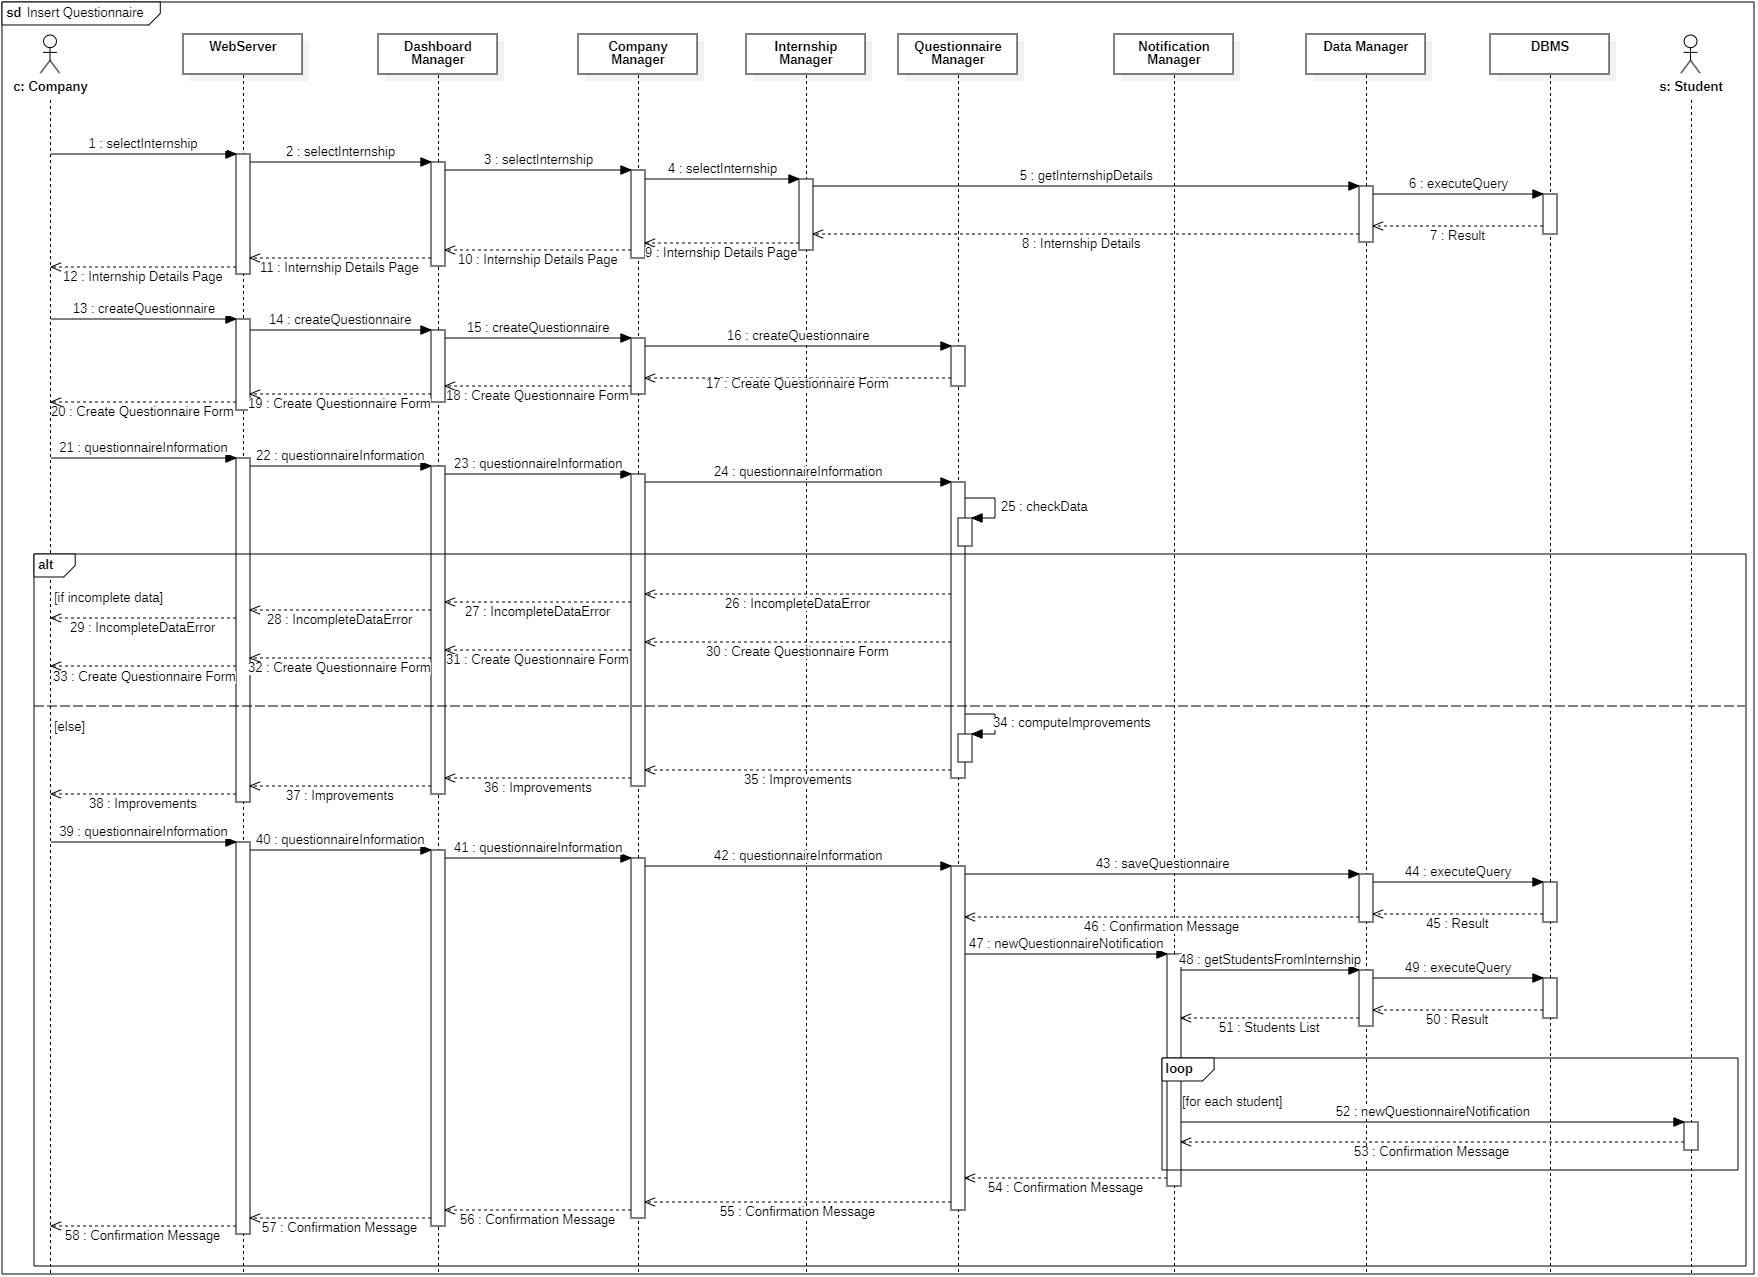
\includegraphics[width=1\linewidth]{DD/Images/Runtime Sequence Diagram Images/insert_questionnaire.png}
    \caption{Diagram for [UC9]}
    \label{fig: Insert Questionnaire Diagram}
\end{figure}

This diagram shows the process for a company to create a questionnaire for an internship. The company begins by selecting the internship and accessing the questionnaire creation form. They input the questions and structure of the questionnaire and submit it for validation. The system checks the data for completeness and correctness, displaying errors if necessary. For valid inputs, improvement suggestions are provided to enhance the questionnaire. Once finalized, the questionnaire is saved to the database. Notifications are sent to students associated with the internship, informing them of the new questionnaire and enabling them to respond promptly.

\subsection{Update Questionnaire}
\begin{figure} [H]
    \centering
    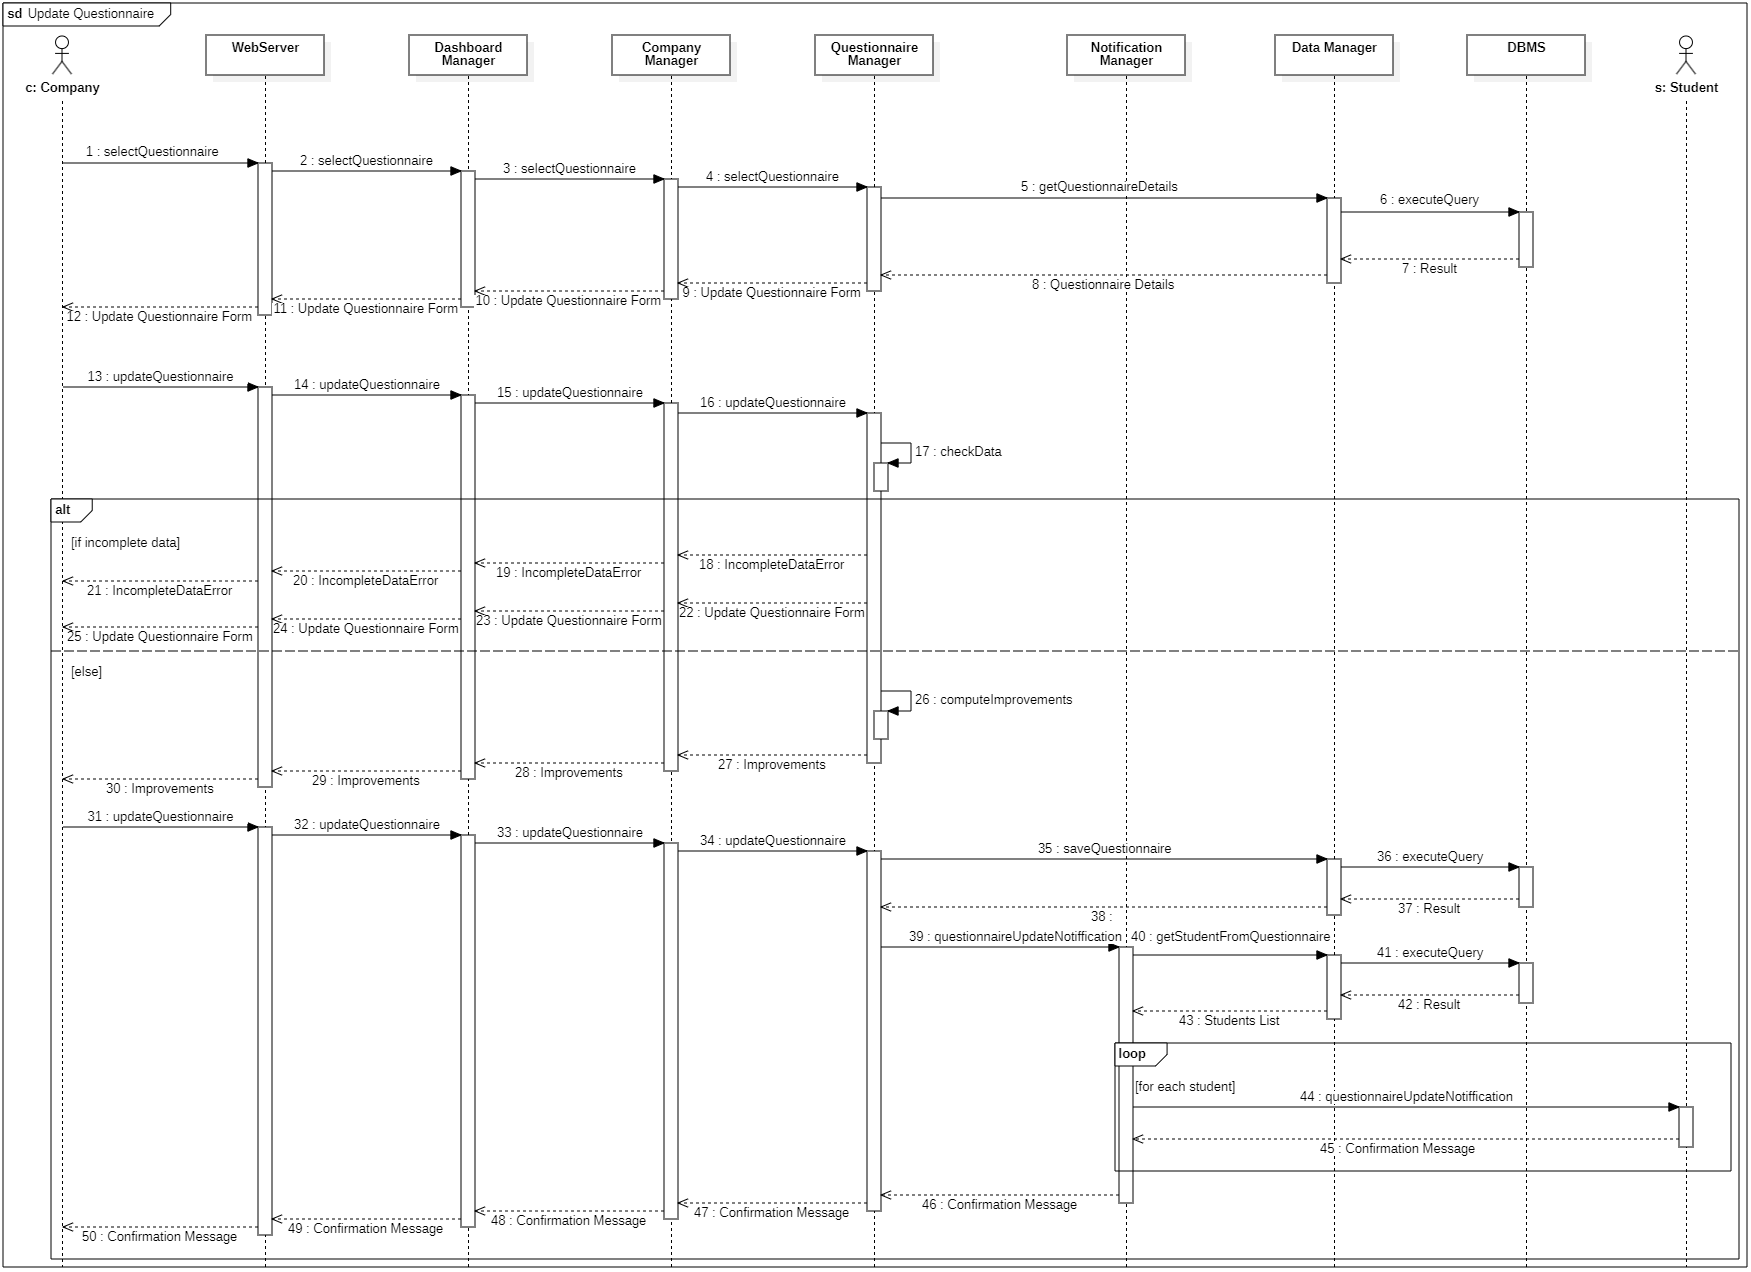
\includegraphics[width=1\linewidth]{DD/Images/Runtime Sequence Diagram Images/update_questionnaire.png}
    \caption{Diagram for [UC10]}
    \label{fig: Update Questionnaire Diagram}
\end{figure}

This sequence diagram explains how a company updates an existing questionnaire linked to an internship. The process starts with the company selecting the questionnaire to edit, and the system retrieves its current details. The company updates the questions or structure and submits the changes. The system validates the new data, displaying errors for incomplete or incorrect inputs. If valid, suggestions for improvement may be offered, such as enhancing clarity or relevance. Once finalized, the updated questionnaire is saved to the database. Notifications are sent to the students associated with the internship, informing them of the updated content to ensure they are aware of the changes.

\subsection{Answer Questionnaire}
\begin{figure} [H]
    \centering
    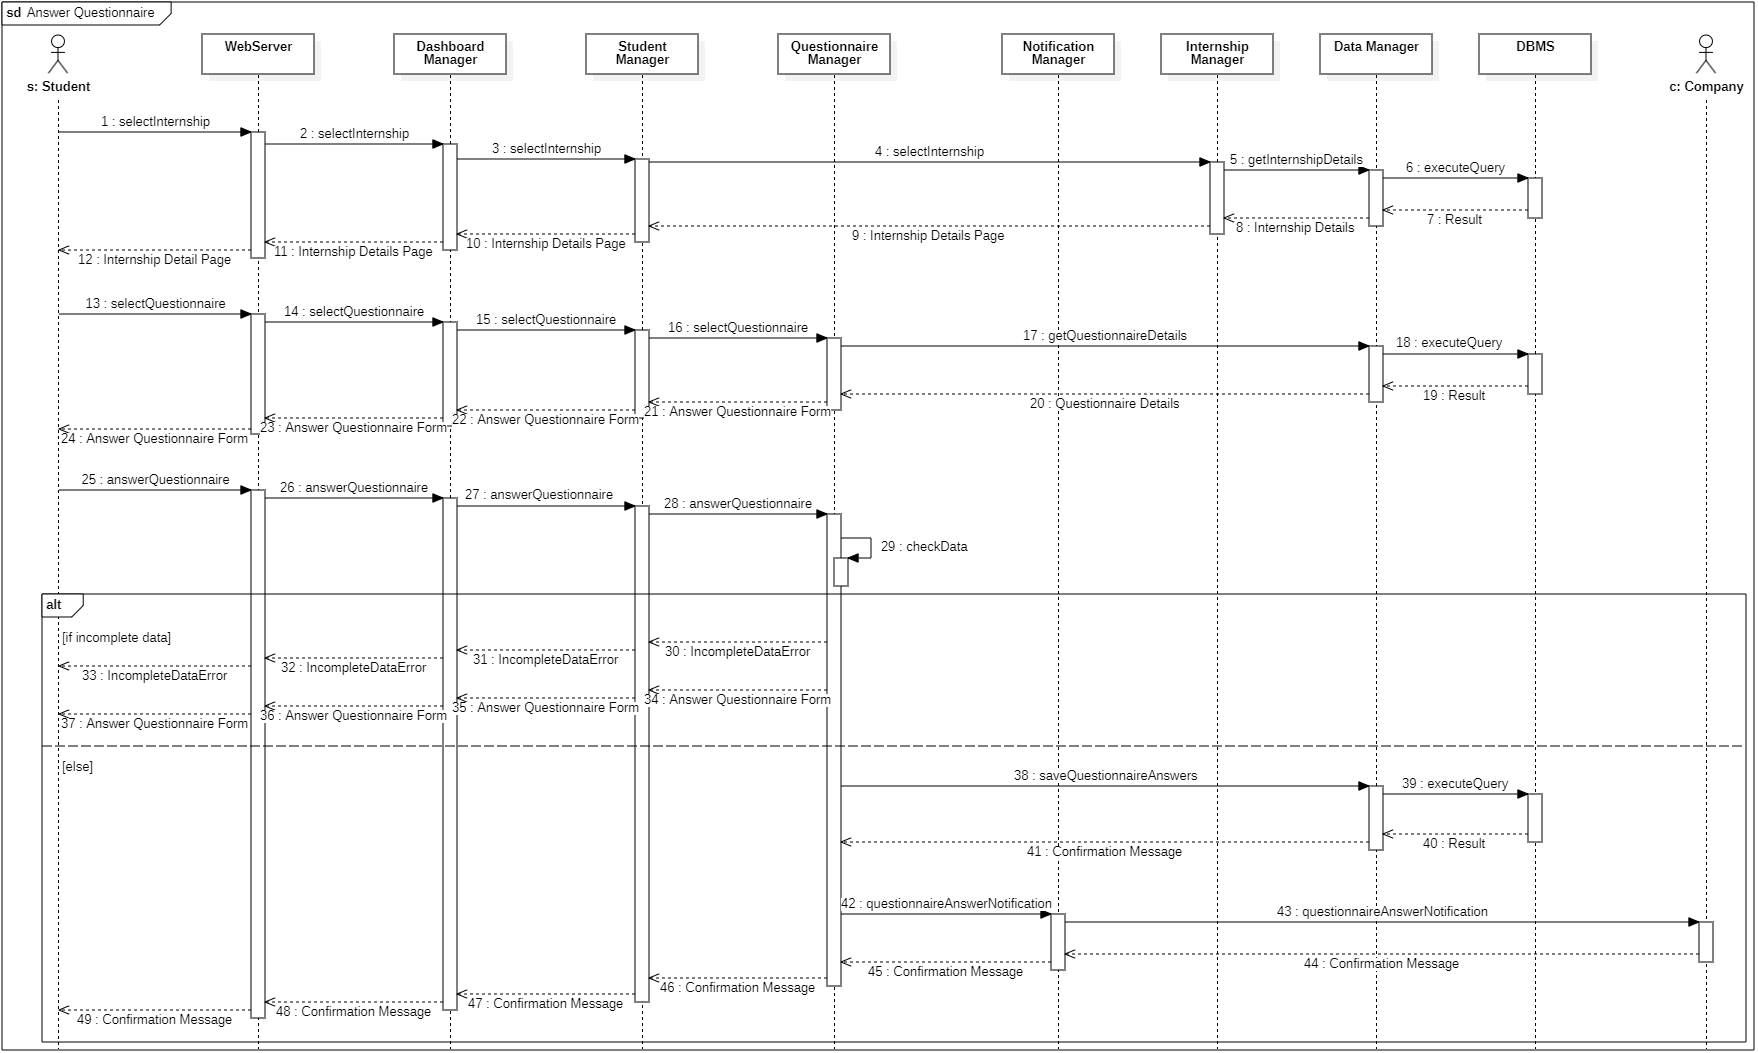
\includegraphics[width=1\linewidth]{DD/Images/Runtime Sequence Diagram Images/answer_questionnaire.png}
    \caption{Diagram for [UC11]}
    \label{fig: Answer Questionnaire Diagram}
\end{figure}
This sequence diagram illustrates the process of a student answering a questionnaire linked to an internship. The student selects an internship, and the system retrieves its details for display. They then select the associated questionnaire and access its form. After completing the questionnaire, the system validates the responses. If there are incomplete or invalid answers, the system prompts the student to correct the input. Once the answers are complete, the system saves the responses to the database. A notification is sent to the company, and the student receives a confirmation message, ensuring the process is completed transparently.

\subsection{Evaluate Application}
\begin{figure} [H]
    \centering
    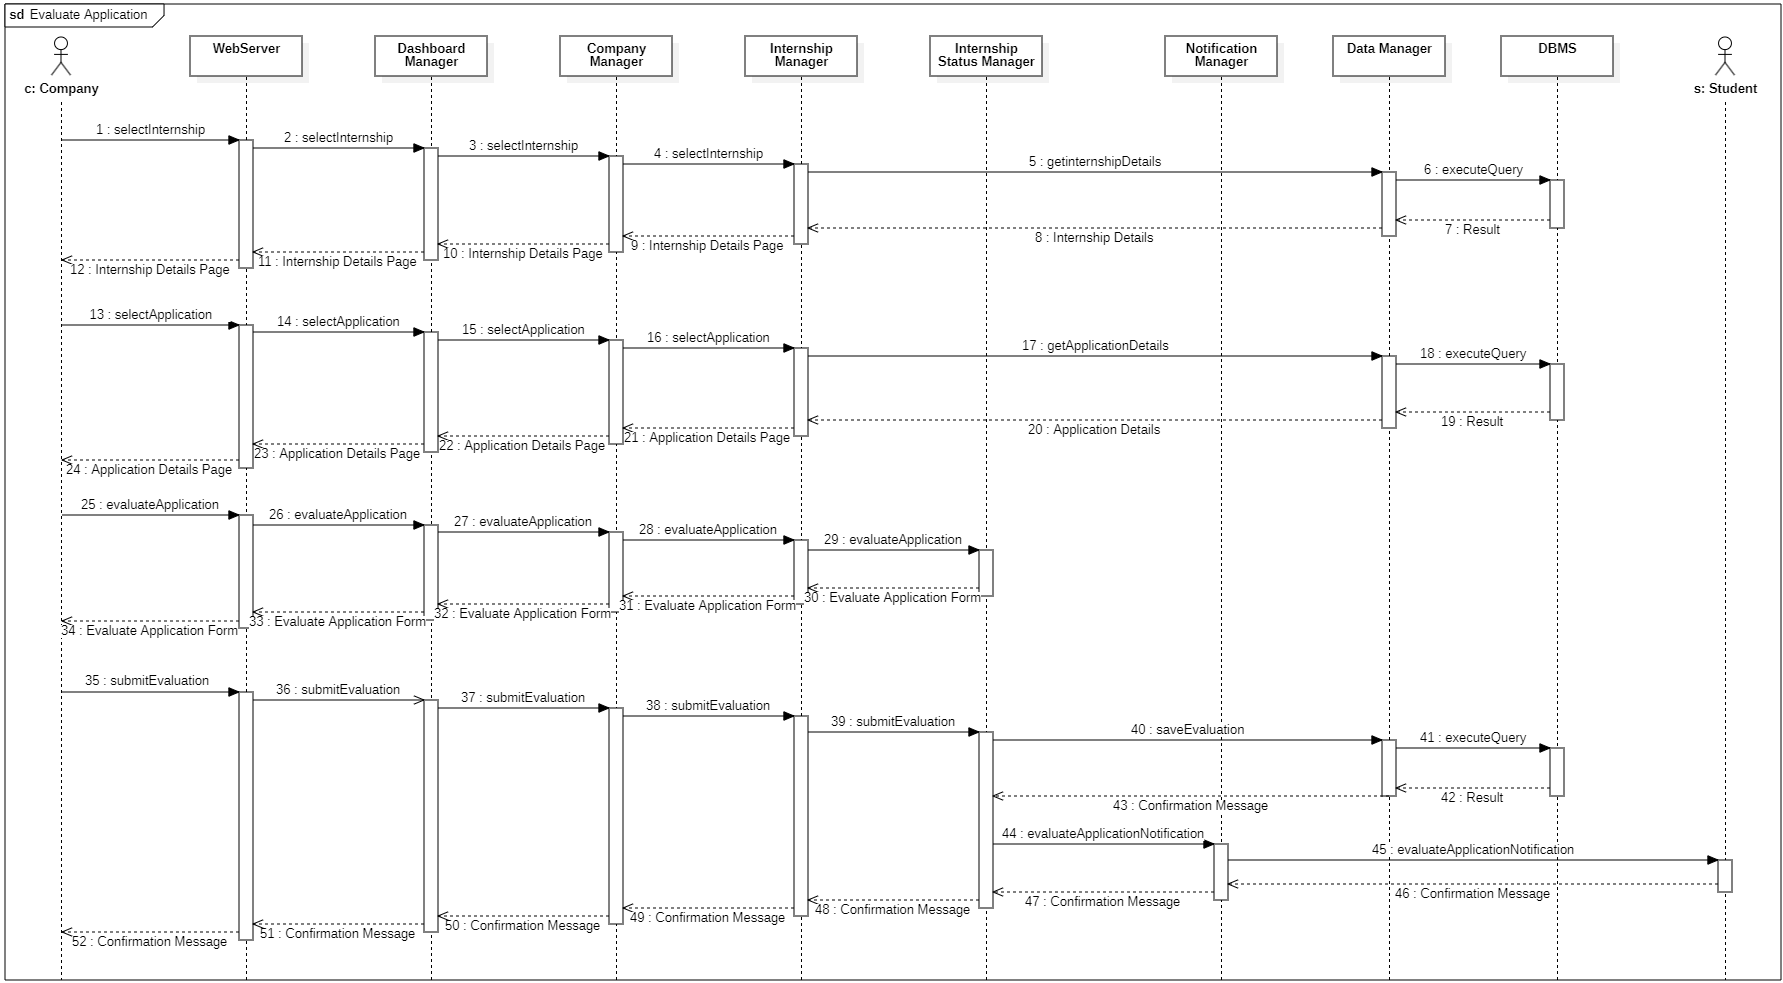
\includegraphics[width=1\linewidth]{DD/Images/Runtime Sequence Diagram Images/evaluate_application.png}
    \caption{Diagram for [UC12]}
    \label{fig: Evaluate Application Diagram}
\end{figure}
This sequence diagram illustrates the process by which a company evaluates a student’s application for an internship. The process begins when the company selects the internship for which they want to evaluate applications, and the system retrieves the relevant details. The company then selects a specific application from the list, and the system fetches its details for review. After reviewing the application, the company accesses the evaluation form, where they provide feedback or a decision (e.g., accept or reject). The system validates the evaluation and saves it to the database. A notification is sent to the student regarding the outcome, and the company receives a confirmation message, ensuring transparency and effective communication.

\subsection{Monitor Internship}
\begin{figure} [H]
    \centering
    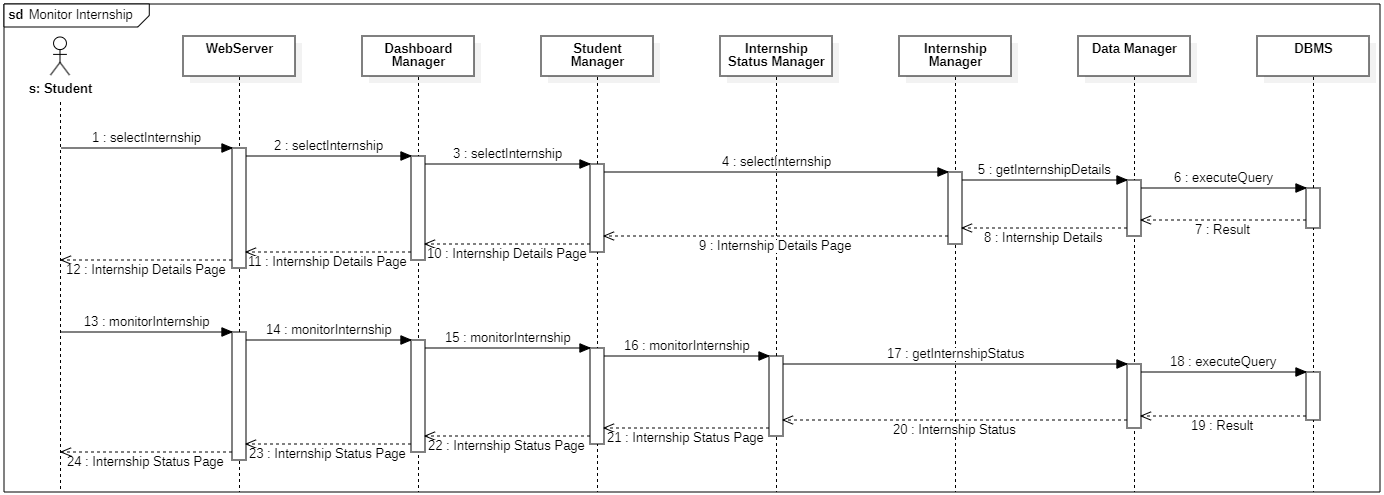
\includegraphics[width=1\linewidth]{DD/Images/Runtime Sequence Diagram Images/monitor_internship.png}
    \caption{Diagram for [UC13]}
    \label{fig: Monitor Internship Diagram}
\end{figure}
This diagram illustrates how a student monitors their internship's status. The student selects their internship from a list and accesses its details. The system retrieves the current status from the database, such as ongoing, completed, or interrupted, and displays it on the monitoring page. This functionality provides students with up-to-date information on their internship progress and any related changes. By making this information accessible, the system ensures students remain informed and can take action if issues arise.

\subsection{Write Feedback}
\begin{figure} [H]
    \centering
    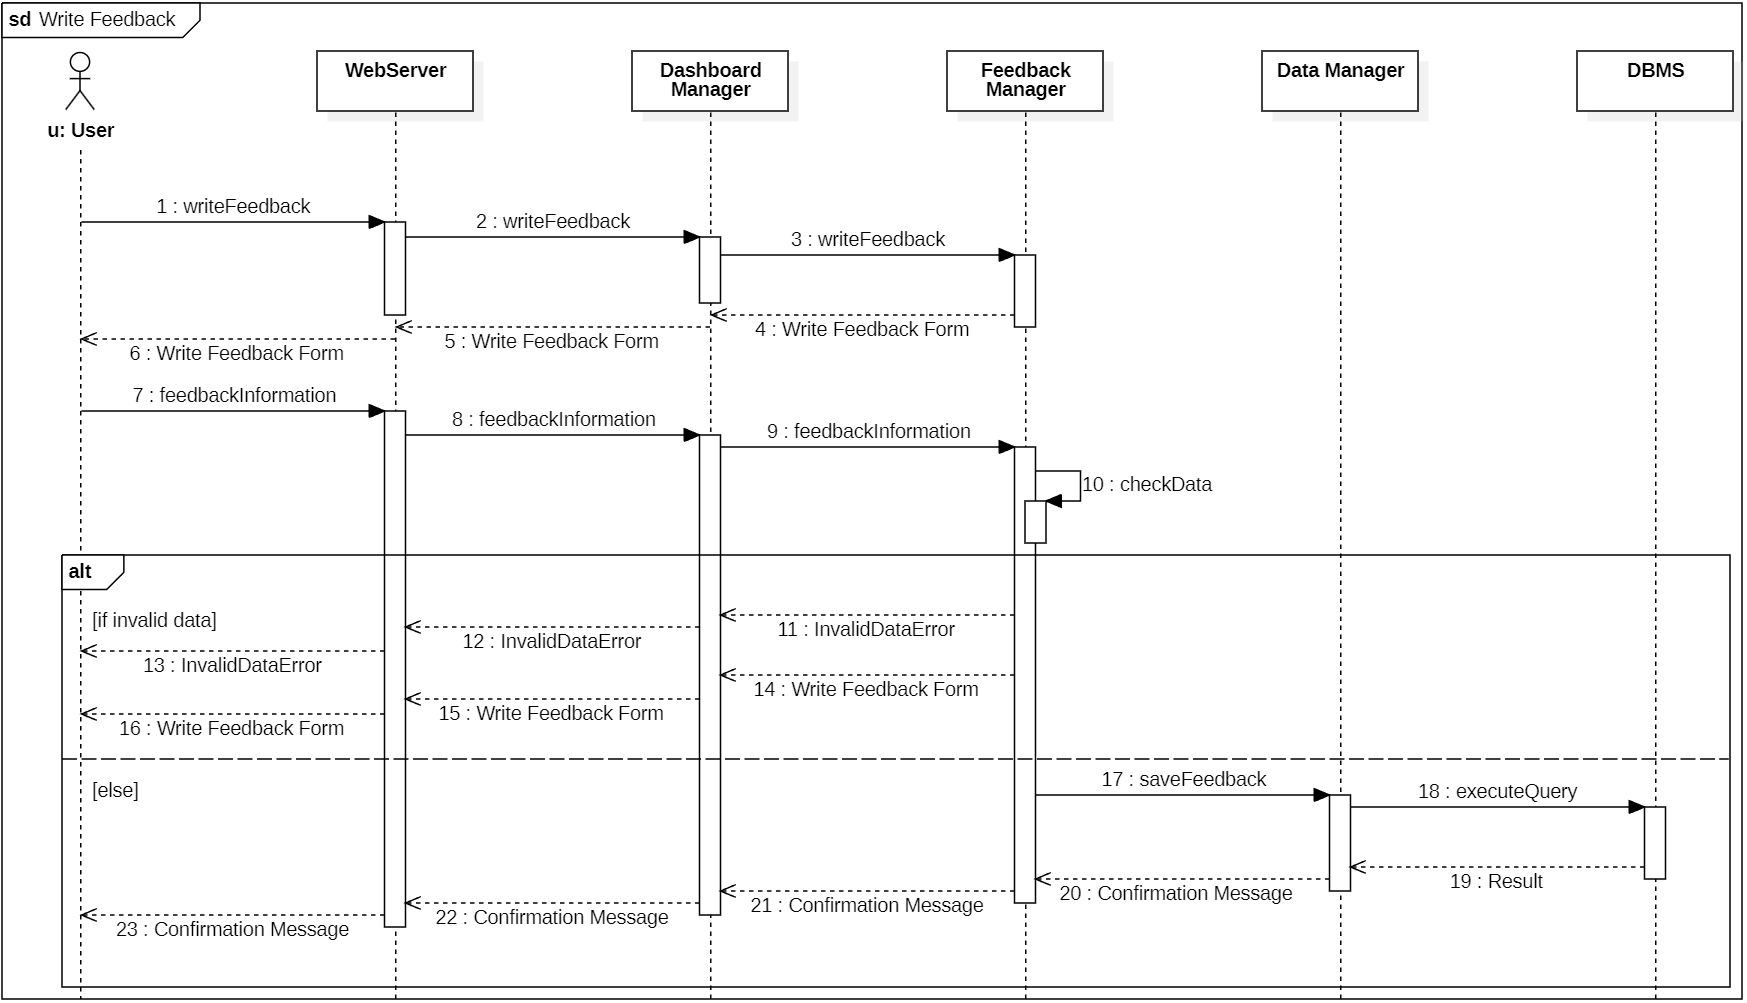
\includegraphics[width=1\linewidth]{DD/Images/Runtime Sequence Diagram Images/write_feedback.png}
    \caption{Diagram for [UC14]}
    \label{fig: Write Feedback Diagram}
\end{figure}

This sequence diagram shows how a user provides feedback on the platform. The user accesses the feedback form and enters details about their experience or suggestions for improvement. The system validates the input for completeness. If the data is incomplete or incorrect, the system prompts the user to revise their input. Once validated, the feedback is saved in the database, and a confirmation message is sent to the user. This feature ensures the platform can collect valuable insights to enhance its functionality and user experience.

\subsection{Write Complaint}
\begin{figure} [H]
    \centering
    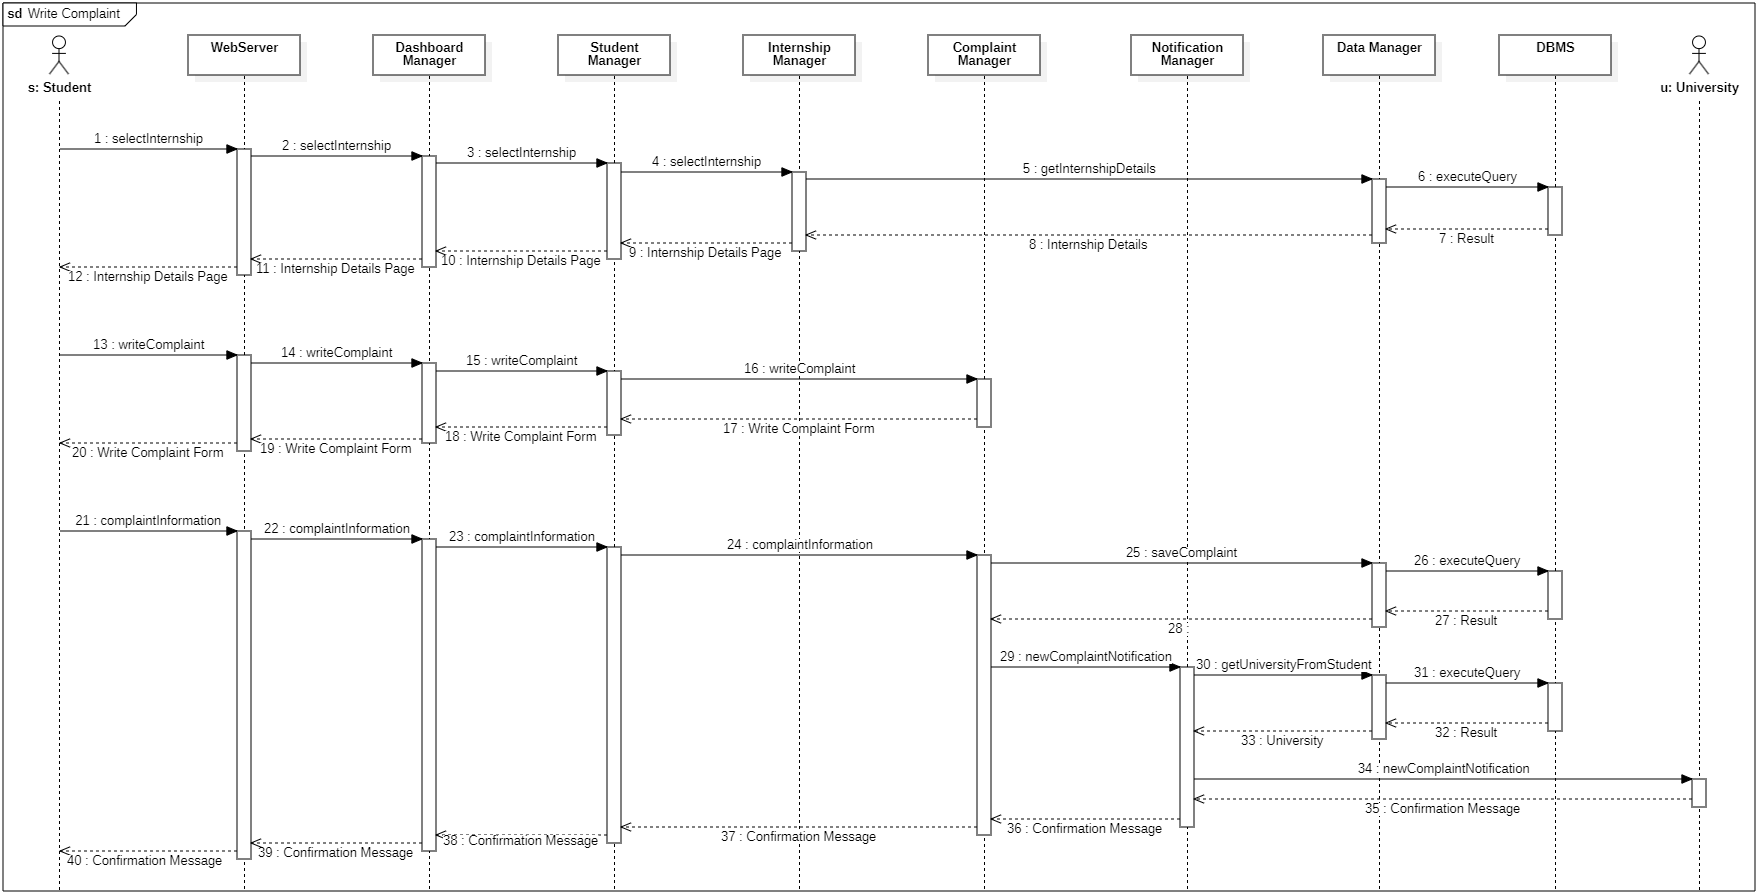
\includegraphics[width=1\linewidth]{DD/Images/Runtime Sequence Diagram Images/write_complaint.png}
    \caption{Diagram for [UC15]}
    \label{fig: Write Complaint Diagram}
\end{figure}

This diagram explains how a student can file a complaint about an internship. The student begins by selecting the relevant internship and viewing its details. They then access the complaint form and input the required information, such as the nature of the complaint and any relevant details. Once submitted, the system validates the data for completeness and accuracy. The complaint is saved in the database and forwarded to the university responsible for the student. Notifications are sent to the student and the university to acknowledge the submission and initiate follow-up actions. This ensures transparency and accountability for resolving issues.

\subsection{Handle Complaint}
\begin{figure} [H]
    \centering
    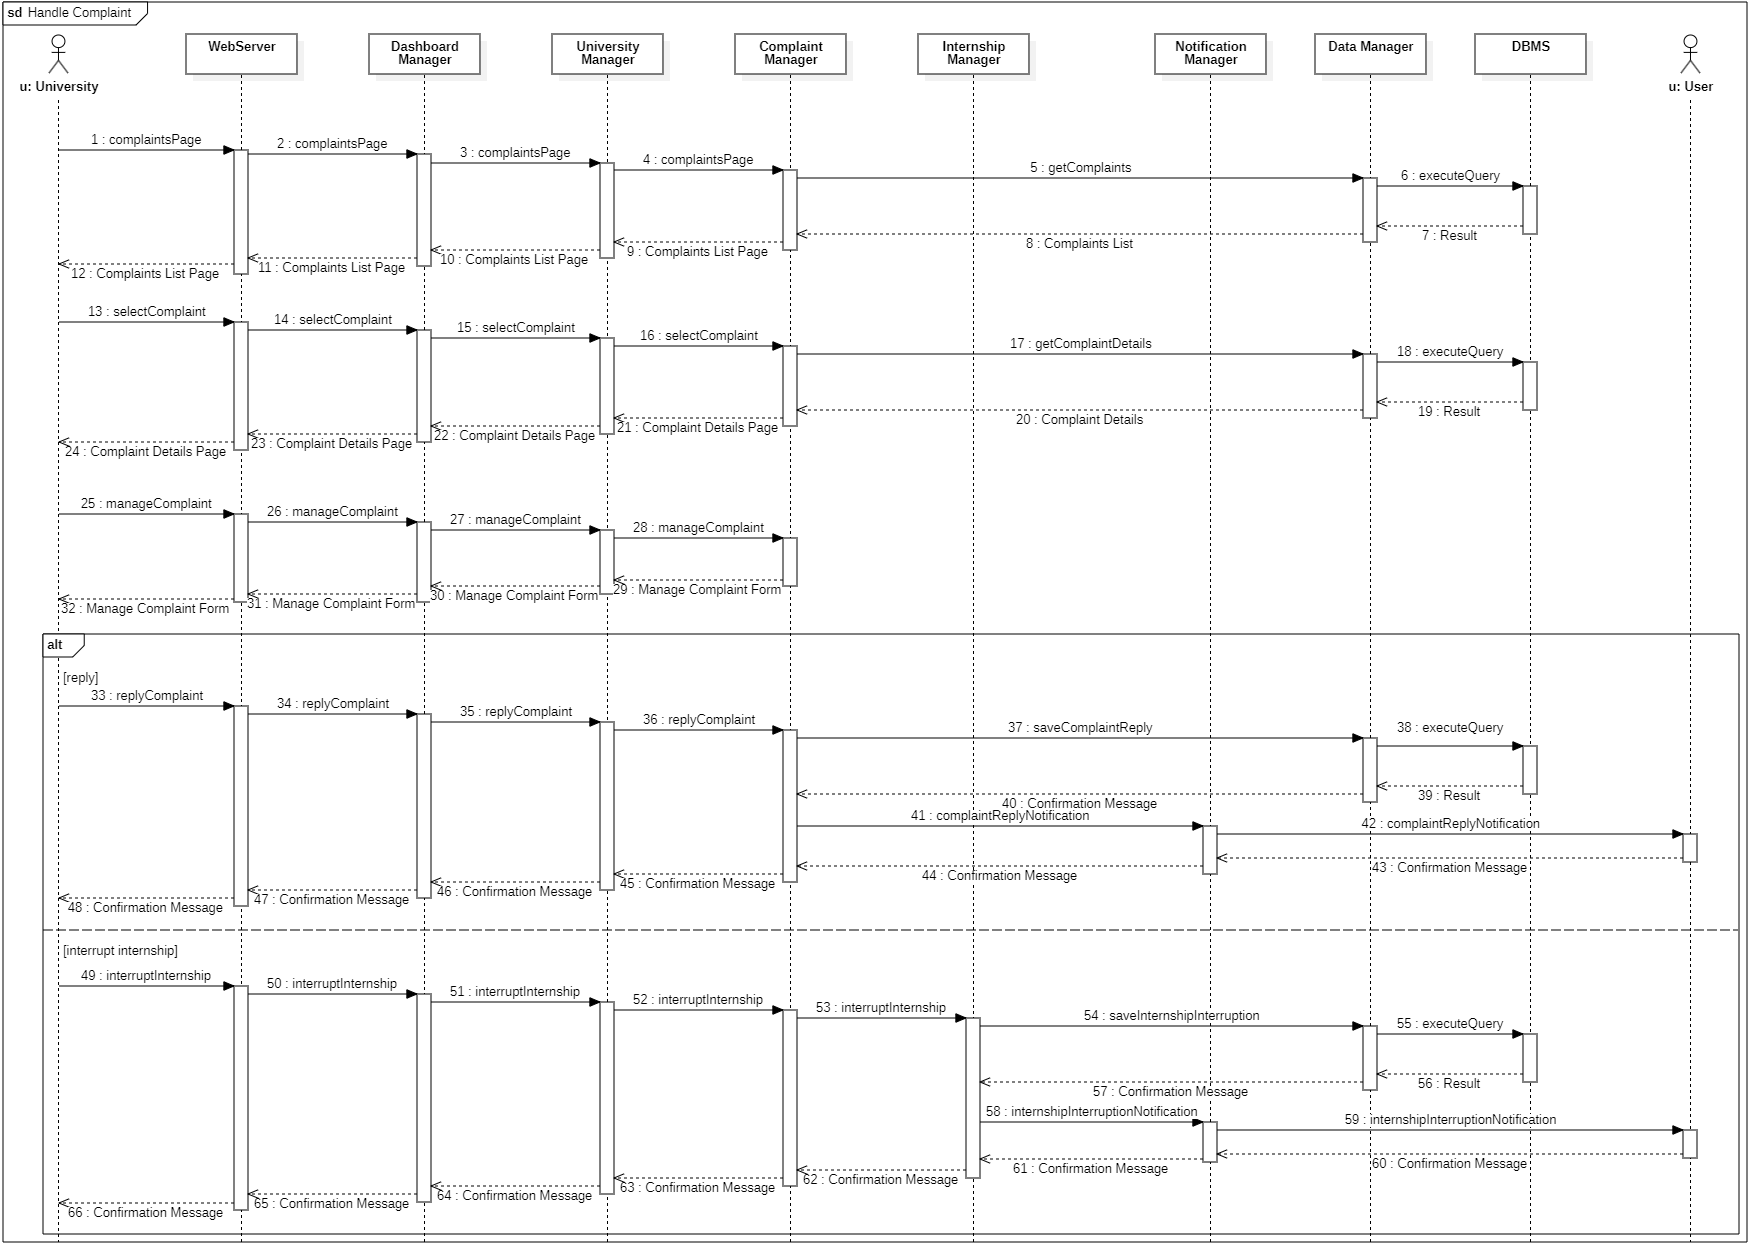
\includegraphics[width=1\linewidth]{DD/Images/Runtime Sequence Diagram Images/handle_complaint.png}
    \caption{Diagram for [UC16]}
    \label{fig: Handle Complaint Diagram}
\end{figure}
This sequence diagram details how a university manages a complaint filed by a student. The university accesses the list of complaints and selects one to view its details. After reviewing the information, they can take action by responding to the complaint or deciding to interrupt the internship. The system validates and saves any actions taken. Notifications are sent to the relevant parties, including the student, company, or internship manager, depending on the resolution. This process ensures complaints are addressed efficiently and transparently, maintaining accountability among all stakeholders.

\newpage
\section{Component Interface}

\subsubsection*{Registration Manager}
\begin{itemize}

    \item \textbf{selectUser}(\textit{Enum userType}) \\
    Selects the type of user (Student, Company or University).

    \item \textbf{registration}(\textit{String name, String surname, String email, String password, int universityId, String universityName}) \\
    Registers a new student with the given details.

    \item \textbf{registration}(\textit{String name, String surname, String email, String password, String companyName}) \\
    Registers a new company with the given details.

    \item \textbf{registration}(\textit{String name, String surname, String email, String password, String universityName}) \\
    Registers a new university with the given details.

    \item \textbf{checkData}(\textit{String email, String password}) \\
    Verifies that the provided email and password meet the required validation rules.

\end{itemize}

\subsubsection*{Login Manager}
\begin{itemize}

    \item \textbf{login}(\textit{String email, String password}) \\
    Logs in a user with the given email and password.

    \item \textbf{checkData}(\textit{String email, String password}) \\
    Verifies that the provided email and password meet the required validation rules.

\end{itemize}

\subsubsection*{Email Manager}
\begin{itemize}

    \item \textbf{verify}(\textit{String email}) \\
    Verifies the provided email address (e.g., sends a confirmation or validation link).

\end{itemize}

\subsubsection*{Internship Manager}
\begin{itemize}

    \item \textbf{createInternship}() \\
    Opens a form used to input details for a new internship.

    \item \textbf{internshipInformation}(\textit{String name, Date deadline, List<Requirement> requirements, String description, String location}) : Internship \\
    Provides comprehensive information about the internship.  
    Returns an \textbf{Internship} object containing all relevant details.

    \item \textbf{computeImprovements}(\textit{Internship internship}) : List<String> \\
    Computes a list of improvements or suggestions to make an internship more appealing.  
    Returns a list of suggested improvements (\textbf{List<String>}).

    \item \textbf{updateInternship}() \\
    Opens a form to update an existing internship.

    \item \textbf{selectInternship}(\textit{String internshipName}) : Internship \\
    Selects a specific internship by its name.  
    Returns the selected \textbf{Internship}.

    \item \textbf{searchInternship}(\textit{Date deadline, List<Requirement> requirements}) : List<Internship> \\
    Searches for internships that match the given criteria.  
    Returns a list of matching \textbf{Internship} objects.

    \item \textbf{interruptInternship}(\textit{String internshipName}) \\
    Interrupts or terminates an ongoing internship given by its name.

    \item \textbf{checkData}(\textit{String name, Date deadline, List<Requirement> requirements, String description, String location}) : boolean \\
    Checks the validity or completeness of the internship data.  
    Returns \textbf{true} if the data is valid, \textbf{false} otherwise.

    \item \textbf{submitApplication}() \\
    Opens a form to submit an application.

    \item \textbf{applicationInformation}(\textit{String text}) : Application \\
    Provides comprehensive information about the application.  
    Returns an \textbf{Application} containing the application details.

    \item \textbf{selectApplication}(\textit{int applicationId}) : Application \\
    Selects a particular application for viewing or processing.  
    Returns the selected \textbf{Application}.

    \item \textbf{evaluateApplication}() \\
    Opens a form to evaluate an existing application.

    \item \textbf{submitEvaluation}(\textit{int applicationId, String decision}) \\
    Submits a final evaluation or decision on an application.

\end{itemize}

\subsubsection*{Questionnaire Manager}
\begin{itemize}

    \item \textbf{createQuestionnaire}() \\
    Opens a form to create a new questionnaire.

    \item \textbf{questionnaireInformation}(\textit{List<String> questions}) : Questionnaire \\
    Provides comprehensive information about the questionnaire.  
    Returns a \textbf{Questionnaire} containing the questions details.

    \item \textbf{computeImprovements}(\textit{Questionnaire questionnaire}) : List<String> \\
    Computes a list of improvements or suggestions to make the questionnaire more appealing.  
    Returns a list of suggested improvements (\textbf{List<String>}).

    \item \textbf{updateQuestionnaire}() \\
    Opens a form to update an existing questionnaire.

    \item \textbf{selectQuestionnaire}(\textit{int questionnaireId}) : Questionnaire \\
    Selects a particular questionnaire by its ID.  
    Returns the selected \textbf{Questionnaire}.

    \item \textbf{answerQuestionnaire}(\textit{List<String> answers}) \\
    Provides answers to a questionnaire.

\end{itemize}

\subsubsection*{Internship Status Manager}
\begin{itemize}

    \item \textbf{monitorInternship}(\textit{String internshipName}) : Status \\
    Provides the status of an internship.  
    Returns the (\textbf{Status}) of the selected internship.

\end{itemize}

\subsubsection*{Complaint Manager}
\begin{itemize}

    \item \textbf{writeComplaint}() \\
    Opens a form to write a new complaint.

    \item \textbf{complaintInformation}(\textit{String text}) : Complaint \\
    Provides details of the complaint.
    Returns a \textbf{Complaint} containing its text.

    \item \textbf{complaintsPage}() \\
    Opens a page listing existing complaints.

    \item \textbf{selectComplaint}(\textit{int id}) \\
    Selects a particular complaint by its ID.

    \item \textbf{manageComplaint}() \\
    Opens a form to manage or respond to a complaint.

    \item \textbf{replyComplaint}(\textit{String text}) \\
    Submits a reply to the selected complaint.

    \item \textbf{interruptInternship}(String internshipName) \\
    Interrupts an internship based on a complaint or issue.

\end{itemize}

\subsubsection*{CV Manager}
\begin{itemize}

    \item \textbf{insertCV}() \\
    Opens a form to insert a new CV.

    \item \textbf{selectCV}() : CV \\  
    Returns the selected \textbf{CV}.

    \item \textbf{updateCV}() \\
    Opens a form to update the CV.

    \item \textbf{CVInformation}(\textit{List<String> cvDetails}) : CV \\
    Provides comprehensive information about a CV.  
    Returns a \textbf{CV} containing all relevant details.

    \item \textbf{checkData}(\textit{CV cv}) : Boolean \\
    Checks the validity or completeness of the CV data.  
    Returns \textbf{true} if the data is valid, \textbf{false} otherwise.

    \item \textbf{computeImprovements}(\textit{CV cv}) : List<String> \\
    Computes a list of improvements or suggestions to make the CV more appealing.  
    Returns a list of suggested improvements (\textbf{List<String>}).

\end{itemize}

\subsubsection*{Feedback Manager}
\begin{itemize}

    \item \textbf{checkData}(\textit{Feedback feedback}) : Boolean \\
    Checks the validity or completeness of the feedback data.  
    Returns \textbf{true} if the data is valid, \textbf{false} otherwise.

    \item \textbf{writeFeedback}() \\
    Opens a form to write a new feedback.

    \item \textbf{feedbackInformation}(\textit{String text}) : Feedback \\
    Provides details of a particular feedback.  
    Returns a \textbf{Feedback} object containing feedback details.

\end{itemize}

\subsubsection*{Notification Manager}
\begin{itemize}

    \item \textbf{internshipUpdateNotification}(\textit{String text}) \\
    Sends a notification about an internship update.

    \item \textbf{newQuestionnaireNotification}(\textit{String text}) \\
    Sends a notification about a new questionnaire.

    \item \textbf{questionnaireUpdateNotification}(\textit{String text}) \\
    Sends a notification about a questionnaire update.

    \item \textbf{questionnaireAnswerNotification}(\textit{String text}) \\
    Sends a notification when a questionnaire is answered.

    \item \textbf{newComplaintNotification}(\textit{String text}) \\
    Sends a notification when a new complaint is submitted.

    \item \textbf{complaintReplyNotification}(\textit{String text}) \\
    Sends a notification about a complaint reply.

    \item \textbf{internshipInterruptionNotification}(\textit{String text}) \\
    Sends a notification that an internship has been interrupted.

    \item \textbf{newApplicationNotification}(\textit{String text}) \\
    Sends a notification about a new application.

    \item \textbf{evaluateApplicationNotification}(\textit{String text}) \\
    Sends a notification about the evaluation of an application.

\end{itemize}

\subsubsection*{Data Manager}
\begin{itemize}

    \item \textbf{checkEmail}(\textit{String email}) : Boolean \\
    Checks whether the given email exists or meets specific criteria.

    \item \textbf{saveStudent}(\textit{Student student}) \\
    Saves a new student record.

    \item \textbf{checkData}(\textit{String email, String password}) : Boolean \\
    Checks the validity of the email and password.

    \item \textbf{saveInternship}(\textit{Internship internship}) \\
    Saves a new internship record.

    \item \textbf{getInternshipDetails}(\textit{String internshipName}) \\
    Retrieves details of an internship by its name.

    \item \textbf{getStudentsFromInternship}(\textit{String internshipName}) : List<Student> \\
    Retrieves a list of students associated with a given internship.

    \item \textbf{getInternships}(\textit{Date deadline, List<Requirement> requirements}) : List<Internship> \\
    Retrieves internships matching certain criteria.

    \item \textbf{saveQuestionnaire}(\textit{Questionnaire questionnaire}) \\
    Saves a new questionnaire.

    \item \textbf{getQuestionnaireDetails}(\textit{int questionnaireId}) \\
    Retrieves details of a questionnaire by its ID.

    \item \textbf{getStudentFromQuestionnaire}(\textit{int questionnaireId}) : List<Student> \\
    Retrieves a list of students linked to a given questionnaire.

    \item \textbf{saveQuestionnaireAnswers}(\textit{String studentName, List<String> answers}) \\
    Saves the answers to a questionnaire for a specific student.

    \item \textbf{getInternshipStatus}(\textit{String internshipName}) : Status \\
    Retrieves the status of an internship.

    \item \textbf{saveComplaint}(\textit{Complaint complaint}) \\
    Saves a new complaint record.

    \item \textbf{getUniversityFromStudent}(\textit{String studentName}) : University \\
    Retrieves the university linked to a given student.

    \item \textbf{getComplaints}(\textit{String universityName}) : List<Complaint> \\
    Retrieves a list of complaints associated with a specific university.

    \item \textbf{getComplaintDetails}(\textit{int complaintId}) : Complaint \\
    Retrieves details of a complaint by its ID.

    \item \textbf{saveComplaintReply}(\textit{String text, String recipient, String author}) \\
    Saves a reply to a complaint, including the recipient and author.

    \item \textbf{saveInternshipInterruption}(\textit{String internshipName, String reason}) \\
    Logs an internship interruption event.

    \item \textbf{saveCV}() \\
    Saves a CV record.

    \item \textbf{saveFeedback}() \\
    Saves a feedback entry.

    \item \textbf{saveApplication}() \\
    Saves a new application record.

    \item \textbf{getApplicationDetails}(\textit{int applicationId}) \\
    Retrieves information about an application.

    \item \textbf{saveEvaluation}() \\
    Saves an evaluation or decision about an application.

\end{itemize}

\newpage
\section{Selected architectural styles and patterns}

This application will be developed using a 3-Tier architecture, which organizes the software into three logical and physical layers. Each tier operates on its own infrastructure, reducing system complexity, and increasing both flexibility and scalability. Moreover, each tier can be developed in parallel by separate teams and can be updated or scaled independently without impacting the other tiers.

\subsubsection*{3-Tier Architecture}

\begin{itemize}
    \item \textbf{Presentation Tier}: \\
    This top-level tier directly interacts with the Users, collecting input and displaying outputs generated by the lower tiers.
    \item \textbf{Application Tier}:\\
    This middle-tier processes requests arriving from the Presentation Tier, performing any required computation. It may also query or update data from the Data Tier, then combine and process the returned data to complete the tasks requested by Users. As it may need to handle multiple concurrent requests, this tier must guarantee data security and integrity.
    \item \textbf{Data Tier}:\\
    The lowest tier, which manages, retrieves, and stores data. It provides interfaces so that the Application Tier can effectively work with the underlying data.
\end{itemize}

\subsubsection*{Client-Server Interactions}

The system largely follows a client-server architecture:
\begin{itemize}
    \item The \textbf{client} is the front-end user interface, serving as the link between the end users and the system.
    \item The \textbf{server} is the back-end platform, receiving user requests, performing necessary computations, and returning the results.
\end{itemize}

In a pure client-server model, the client typically initiates requests, and the server—acting as a passive element—processes and returns the requested data or responses. However, some features require the server to be proactive, such as sending notifications or interacting with external tools without a direct client request. In these cases, the server adopts a more event-driven or active role.

\subsubsection*{Model-View-Controller (MVC) Pattern}

The application’s internal structure follows the MVC pattern, a design principle that divides the software into three interconnected components:

\begin{enumerate}
    \item \textbf{Model}:\\
    Contains methods for handling data—saving, retrieving, and manipulating information from the database.
    
    \item \textbf{View}:\\
    Manages how data is visually represented to the end user. It specifies the layout and user interface elements displayed.
    
    \item \textbf{Controller}:\\
    Serves as the link between the View and the Model. It intercepts user interactions (e.g., button clicks) from the View, executes the necessary operations, and ensures the appropriate data and responses flow between Model and View.
\end{enumerate}

By combining a 3-Tier architecture, a client-server approach, and the MVC pattern, the system ensures modularity, maintainability, and scalability, all while providing a coherent separation of concerns and clear communication between components.


\newpage
\section{Other Design Decisions}

\subsection{Availability}

The introduction of load balancing and replication mechanisms significantly enhances the reliability and availability of the S\&C system. Load balancing optimizes resource utilization by distributing incoming requests evenly across servers, thereby preventing performance bottlenecks. Concurrently, replication ensures fault tolerance by duplicating essential data and services. This redundancy reduces the impact of potential failures and enables the system to maintain consistent data management and service availability even under challenging conditions.

\subsection{Scalability}

A microservices architecture is intentionally designed to be both independently deployable and inherently scalable. Each microservice can be deployed and updated autonomously, thereby preventing disruptions to the entire system when modifications are made. Furthermore, microservices empower the S\&C platform to handle increasing demands by efficiently scaling specific services as needed.

\subsection{Notification Handling}

Notification management is crucial in the S\&C system, affecting every stage of the internship life cycle, from creation to ongoing tracking and completion. Notifications are orchestrated to reach users upon login, or, if a user is already logged in, immediately as they become available. This approach ensures that students, companies, and universities receive timely updates on key events, such as new internship postings, interview schedulings, or feedback requests.

\subsection{Ease of Deployment}

Adopting a microservices strategy also provides significant advantages in terms of deployment. Individual services can be updated independently, allowing direct rollouts without impacting the entire system. In case any issues arise, the microservices approach simplifies diagnosing, isolating, and correcting problems—no need to halt the full platform. This deployment flexibility not only accelerates the release of updates but also boosts resilience and agility, enabling efficient troubleshooting and maintenance.

\subsection{Data Storage}

To streamline operations and simplify data management, the S\&C system employs a unified DBMS that contains information about students, companies, universities, internships, and any additional data relevant to matching or recommendation processes. Centralizing this data reduces the time and complexity associated with retrieval and updates, leveraging the interrelated nature of these components.
